\documentclass[conference]{IEEEtran}
\IEEEoverridecommandlockouts

% Paquetes:
\usepackage{cite}
\usepackage{amsmath,amssymb,amsfonts}
\usepackage{algorithmic}
\usepackage{graphicx}
\usepackage{textcomp}
\usepackage{xcolor}
\usepackage{hyperref}
\usepackage{minted}     % Códigos
\def\BibTeX{{\rm B\kern-.05em{\sc i\kern-.025em b}\kern-.08em
    T\kern-.1667em\lower.7ex\hbox{E}\kern-.125emX}}
\graphicspath{{Figuras/}}


\begin{document}
\title{Trabajo Práctico N°1: Análisis y Diseño de un Acoplamiento Inter-etapa con un Circuito LC}

\author{\IEEEauthorblockN{Monja, Ernesto Joaquín}
\IEEEauthorblockA{\textit{Ingeniería Electrónica, Cátedra de Electrónica Analógica III} \\
                  \textit{Facultad de Ciencias Exactas, Físicas y Naturales (FCEFyN)} \\
                          Córdoba, Argentina \\
                          ernesto.monja@mi.unc.edu.ar}}
\maketitle

\begin{abstract}
El documento describe el proceso de diseño, simulación y armado físico de un acoplamiento inter-etapa mediante una red LC, la cual provee una función de sintonía como adaptación de impedancia. 
\end{abstract}



\section{Introducción}
El objetivo principal de este trabajo práctico consiste en sintetizar los componentes reactivos de una red LC paralelo para el acople inter-etapa de un sistema de recepción de radiofrecuencias.



\section{Desarrollo}
\subsection{Marco Teórico}
Se comenzó el análisis partiendo de una red LC paralelo, la cual como indica la Fig. \ref{fig:fig_1}, se conectó entre el generador y la carga.

\begin{figure}[htbp]
    \centering
    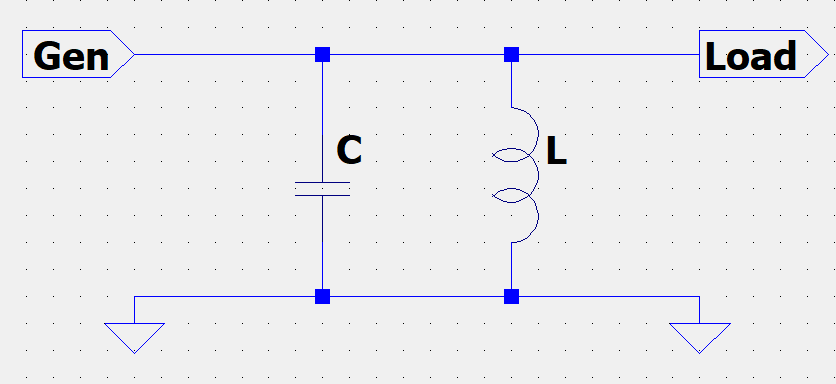
\includegraphics[width=1\linewidth]{Figura 1.png}
    \caption{Acoplador $LC$.}
    \label{fig:fig_1}
\end{figure}

Una red LC como la presentada, tiene la particularidad de actuar como un filtro pasabanda, para la cual se puede variar tanto el ancho de banda ($BW$) como la frecuencia central del filtro, ajustando sus parámetros eléctricos. Se tiene que una característica fundamental de esta red LC, es que existe una frecuencia donde tanto las reactancias capacitivas e inductiva se cancelan entre sí. A esta frecuencia se la conoce como frecuencia de resonancia ($f_{0}$) y se define como:
\begin{equation}
    f_{0} = \frac{1}{2\pi\sqrt{LC_{T}}}
    \label{eq_1}
\end{equation}

Se puede definir también al factor de calidad cargado de este circuito como la relación :
\begin{equation}
    Q_{C} = \frac{f_{0}}{BW} = \frac{R_{T}}{X_{L}}
    \label{eq_2}
\end{equation}

Donde se define a $R_{T}$ como la resistencia total del circuito y está dada por: $R_{T} = R_{G}//R_{P}//R_{L}$, donde $R_{G}$ es la resistencia del generador, $R_{P}$ es la resistencia de pérdida del inductor y $R_{L}$ es la resistencia de carga o de entrada del amplificador que se conecta luego del acoplador. Se sabe también que $X_{L}$ será igual a $X_{L} = 2 \pi f_{0} L$.

Si bien se cumple la propiedad de sintonía del acoplador, se necesitó que esta red genere una adaptación de impedancias. Para ello se propuso dividir primero la capacidad $C_T$ en dos capacidades iguales de valor $\frac{C_{T}}{2}$ conectadas en paralelo, de modo que el circuito quedó como el que se muestra en la Fig. \ref{fig:fig_2}.

\begin{figure}[htbp]
    \centering
    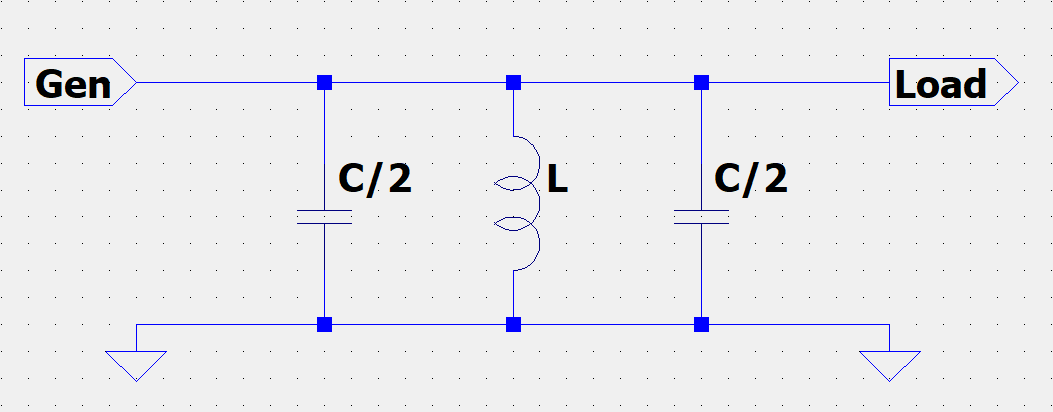
\includegraphics[width=1\linewidth]{Figura 2.png}
    \caption{Acoplador $LC$ con 2 capacitores.}
    \label{fig:fig_2}
\end{figure}

Luego, se puede dividir cada uno de estos 2 capacitores, en otros 2 capacitores en serie por cada rama del paralelo, de modo que el acoplador tiene la forma que se muestra en la Fig. \ref{fig:fig_3}.

\begin{figure}[htbp]
    \centering
    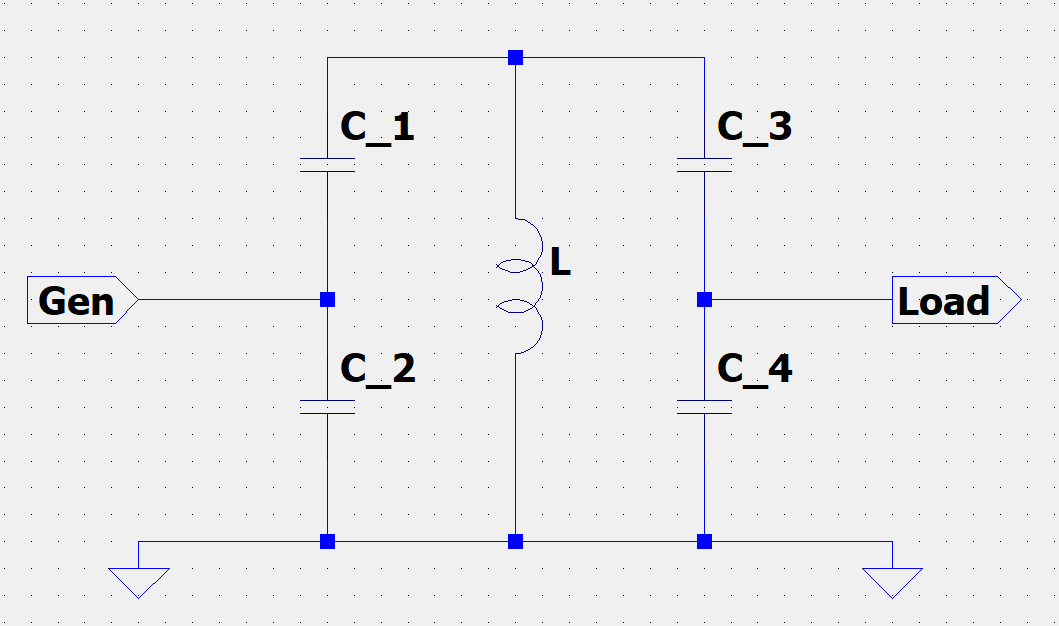
\includegraphics[width=1\linewidth]{Figura 3.png}
    \caption{Acoplador $LC$ con 4 capacitores.}
    \label{fig:fig_3}
\end{figure}

Se deduce que estas capacidades deberán ser iguales a:
\begin{equation}
    \frac{C_{T}}{2} = \frac{C_{1}C_{2}}{C_{1} + C_{2}}
    \label{eq_3}
\end{equation}
\begin{equation}
    \frac{C_{T}}{2} = \frac{C_{3}C_{4}}{C_{3} + C_{4}}
    \label{eq_4}
\end{equation}

Nótese que aquí la capacidad total del circuito sigue siendo la misma, de modo tal que la frecuencia de resonancia descrita en \eqref{eq_1} se mantiene igual, sin embargo se implementó intencionalmente un transformador capacitivo mediante estas 4 capacidades. Esto nos permitió introducir el concepto de reflexión de impedancias $R_{in}$ y $R_{L}$ hacia dentro del circuito, facilitando así los cálculos.

Para demostrar las relaciones de transformación de impedancia, se realizó el análisis considerando únicamente el puerto de entrada, de modo que la demostración para el puerto de salida es prácticamente igual a la del puerto de entrada. Por lo tanto, si se define a la tensión que se encuentra en el borne superior de $C_{1}$ y tierra como $V_0$, entonces se debe cumplir que:
\begin{equation}
    V_{G} = V_{0} \frac{Z_{C_{2}}}{Z_{C_{1}} + Z_{C_{2}}} = V_{0} \frac{\frac{1}{sC_{2}}}{\frac{1}{sC_{1}} + \frac{1}{sC_{2}}}
    \label{eq_5}
\end{equation}

Multiplicando numerador y denominador por $sC_{2}C_{1}$, se tiene que:
\begin{equation}
    V_{G} = V_{0} \left(\frac{C_{1}}{C_{1} + C_{2}}\right) = V_{0}(k)
    \label{eq_6}
\end{equation}

Nótese la similitud que comparte este divisor capacitivo con un auto transformador, donde la única diferencia yace en que se usan capacitores en lugar de inductores. Se tiene entonces que se puede definir a la relación de transformación $k$ tal cual como se ha descrito en \eqref{eq_6}.

Al igual que un transformador, donde se tiene que al analizar las impedancias del primario, estas pueden ser reflejadas al secundario del mismo si se las multiplica por $\frac{1}{k^{2}}$ \cite{B1}, se tiene que para el transformador capacitivo ocurre exactamente lo mismo, de modo que se cumple que:
\begin{equation}
    R_{G}' = \frac{R_{G}}{\left(\frac{C_{1}}{C_{1} + C_{2}}\right)^{2}} = R_{G} \left(1 + \frac{C_{2}}{C_{1}}\right)^{2}
    \label{eq_7}
\end{equation}

Como se mencionó anteriormente, el análisis es prácticamente igual para el puerto de salida de modo que la relación de reflexión de impedancias para la salida esta dada por:
\begin{equation}
    R_{L}' = \frac{R_{L}}{\left(\frac{C_{3}}{C_{3} + C_{4}}\right)^{2}} = R_{L} \left(1 + \frac{C_{4}}{C_{3}}\right)^{2}
    \label{eq_8}
\end{equation}



\subsection{Cálculo del Inductor y las Capacitancias}                       
Una vez desarrollado el marco teórico, se tienen las herramientas matemáticas principales para comenzar el diseño del inductor y consecuentemente de los capacitores que conformarán a la red de acople. Para ello, se realizó dentro de un repositorio de GitHub, un \href{https://github.com/ErnestMonja/Electronica_Analogica_III/blob/main/Trabajo%20Pr%C3%A1ctico%20N%C2%B01%20-%20Circuitos%20Sintonizados/TP1%20-%20Script%20de%20Inductor-Capacitores%20(Final).ipynb}{código en Python} \cite{B2} que desarrolla el cálculo matemático y detallado en una serie de 11 pasos los cuales se explican de forma breve a continuación:

\begin{itemize}
    \item \underline{Paso 1:} Se definió primeramente la frecuencia de resonancia del filtro y el ancho de banda del circuito en base a \eqref{eq_2}. Estos valores son datos de la consigna del TP1 y son iguales a:
        \begin{equation}
            f_{0} = 18 \ [MHz]
            \label{eq_9}
        \end{equation}
        \begin{equation}
            Q_{C} = 10
            \label{eq_10}
        \end{equation}
    
    \item \underline{Paso 2:} Se armó una serie de arreglos y variables individuales en Python que contienen los parámetros físicos mas importantes a la hora de diseñar un inductor, entre ellos:
    \begin{itemize}
        \item \underline{Diámetro del cobre esmaltado ($d_{C}$):} Se tomaron una serie de valores desde $0.08 \ [cm]$ hasta $0.23 \ [cm].$
        
        \item \underline{Separación entre espiras ($S$):} Por una comodidad constructiva, se optó que: 
        \begin{equation}
            S = d_{C}
            \label{eq_11}
        \end{equation}
        
        \item \underline{Diámetro interno del inductor ($D_{0}$):} Para enrollar la bobina, se utilizó un slide de guitarra \cite{B3} de un diámetro de:
        \begin{equation}
            D_{0} = 2.2 \ [cm]
            \label{eq_12}
        \end{equation}
        
        \item \underline{Diámetro total del inductor ($D_{T}$):} Consiste en la suma del diámetro del cobre esmaltado y el diámetro interno del conductor, es decir:
        \begin{equation}
            D_{T} = D_{0} + 2d_{C}
            \label{eq_13}
        \end{equation}
        
        \item \underline{Relación de aspecto ($\frac{l}{D_{T}}$):} Se busca diseñar un inductor lo más cuadrado posible, tal que se tomó una relación de aspecto de entre $1$ a $2$.
        
        \item \underline{Largo del inductor ($l$):} Conociendo a $D_{T}$ y a $\frac{l}{D_{T}}$, se despejó fácilmente el largo del inductor como:
        \begin{equation}
            l = \left(\frac{l}{D_{T}}\right) D_{T}
            \label{eq_14}
        \end{equation}
        
        \item \underline{Numero de espiras ($N$):} Se utilizó la siguiente fórmula para deducir el número de espiras:
        \begin{equation}
            N = \frac{l}{2d_{C}}
            \label{eq_15}
        \end{equation}
    \end{itemize}

    \item \underline{Paso 3:} Se imprimió por pantalla algunos valores de los pasos anterior y se armó una tabla inicial de todos los posibles largos del inductor ($l$) y su número de espiras ($N$) de acuerdo a los valores de la relación de aspecto ($\frac{l}{D_T}$) y el diámetro del cobre esmaltado ($d_{C}$).

    \item \underline{Paso 4:} Para no recurrir a las gráficas de la Constante de Nagaoka \cite{B4}, se optó por recurrir a la Fórmula de Wheeler para inductores \cite{B5}, la cual está descrita por:
    \begin{equation}
        L = \frac{0.394 r^{2} N^{2}}{9r + 10l} [\mu Hy]
        \label{eq_16}
    \end{equation}
    Donde $r = \frac{D_{T}}{2} \ [cm]$. Se dedujo de este paso, una tabla con todos los posibles valores de $L$ de acuerdo a la relación de aspecto ($\frac{l}{D_T}$) y el diámetro del cobre esmaltado ($d_{C}$).
    
    \item \underline{Paso 5:} En este paso, se calculó el factor de calidad cargado $Q_{C}$ según \eqref{eq_2} y el factor de calidad descargado del circuito, donde este último esta definido por:
    \begin{equation}
        Q_{D} = 8550 \frac{D_{T} l}{102l + 450} \sqrt{f_{o}}
        \label{eq_17}
    \end{equation}
    Donde $f_{0}$ esta en $[MHz]$ y tanto $D_{T}$ como $l$ están en $[cm]$. Con el valor de $Q_{D}$, se dedujo la resistencia de pérdida del inductor como:
    \begin{equation}
        R_{P} = Q_{D} X_{L} = 2 \pi f_{o} L Q_{D} \ [\Omega]
        \label{eq_18}
    \end{equation}

    \item \underline{Paso 6:} Se tabularon los valores de $Q_{D}$ y consecuentemente $R_{P}$ de acuerdo a la relación de aspecto ($\frac{l}{D_T}$) y el diámetro del cobre esmaltado ($d_{C}$). 

    \item \underline{Paso 7:} Habiendo definido una amplia gama de valores de inductancia, se procedió a calcular el valor de las capacitancias totales que generan que el circuito oscile en la $f_{0}$ definida según \eqref{eq_9}, siguiendo la siguiente fórmula:
    \begin{equation}
        C_{T} = \frac{1}{(2 \pi f_{o})^2 L} \ [F]
        \label{eq_19}
    \end{equation}

    \item \underline{Paso 8:} Con todos los datos obtenidos hasta este paso, se procedió a realizar distintas curvas paramétricas que miden las variaciones de algunas variables respecto a otras, de acuerdo al diámetro del cobre esmaltado ($d_{C}$). Se observan las gráficas mencionadas de este paso en la Fig. \ref{fig:fig_4}.

    \begin{figure}[htbp]
        \centering
        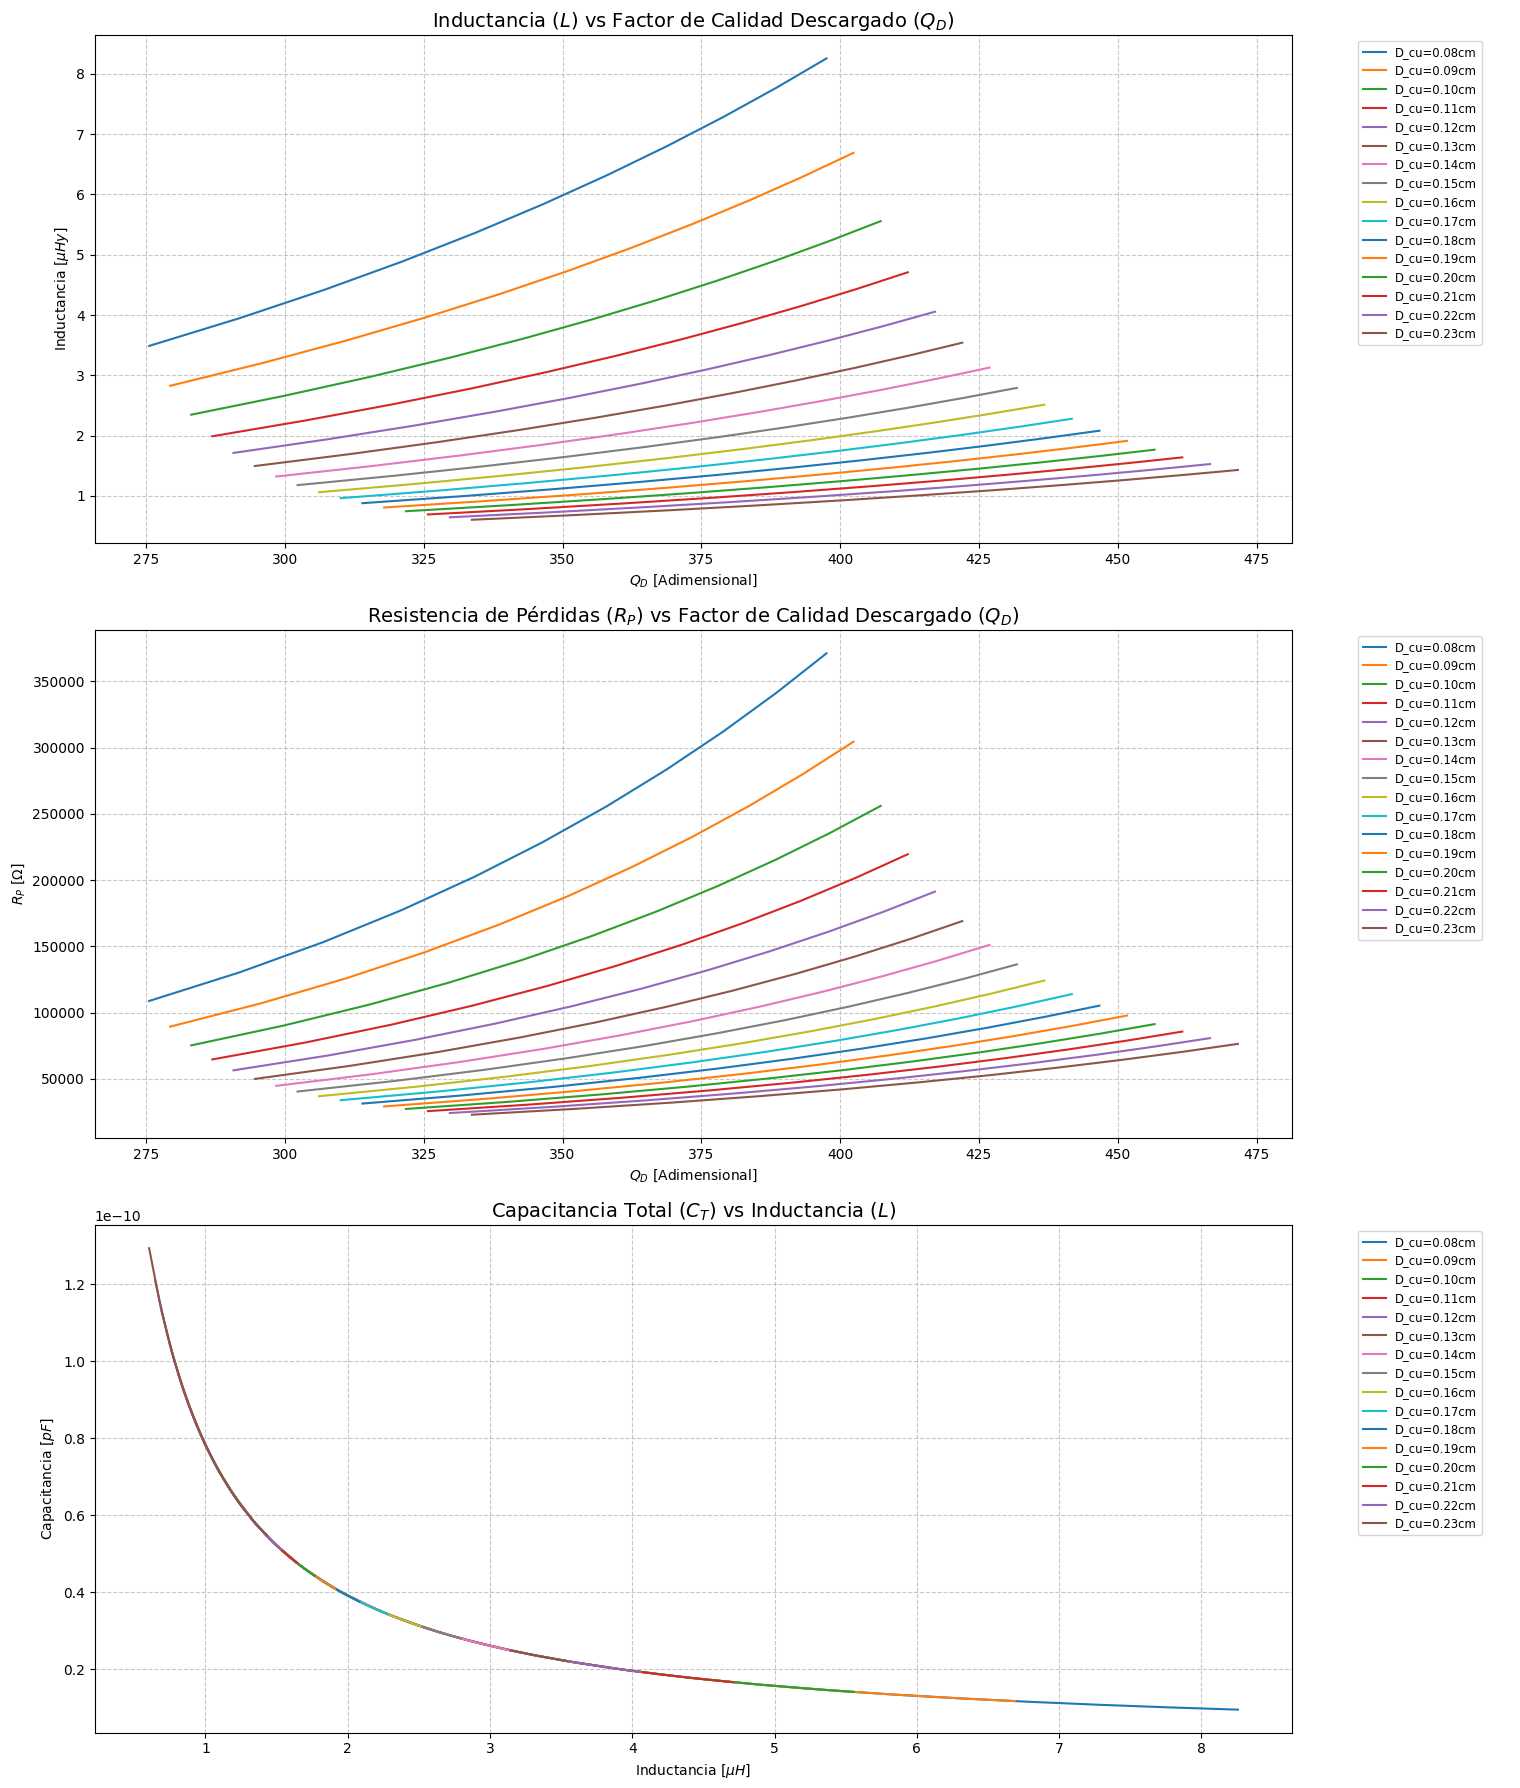
\includegraphics[width=0.9\linewidth]{Figura 4.png}
        \caption{Gráficas de interés para el diseño del inductor.}
        \label{fig:fig_4}
    \end{figure}
    

    \item \underline{Paso 9:} Dado que $Q_{C}$ es dato según \eqref{eq_10}, se calculó entonces la resistencia total del circuito siguiendo \eqref{eq_2} tal que:
    \begin{equation}
        R_{T} = Q_{C} X_{L} = 2 \pi f_{o} L Q_{C}
        \label{eq_20}
    \end{equation}

    \item \underline{Paso 10:} A esta altura del código, se tenían ya todos los parámetros calculados para cada posible par inductor-capacitores de modo que sólo restó elegir el par más conveniente para la construcción física del circuito.
    El algoritmo de filtrado de inductores consistió simplemente en mantener cualquier inductor para el cual, el diámetro del cobre esmaltado se encuentra entre $0.18 \ [cm]$ a $0.2 \ [cm]$. Luego se armó una tabla ordenando cada inductor siguiendo las siguientes reglas:
    \begin{itemize}
        \item Primero se ordenaron de acuerdo a los inductores con una relación de aspecto $\frac{l}{D_{T}}$ más cercana a 1.
        \item Luego si habían 2 o más inductores con misma relación de aspecto, se priorizó al inductor que tenga mayor $Q_{D}$.
    \end{itemize}
    De esta forma, fue posible armar una tabla como la que se muestra en la Fig. \ref{fig:fig_5}
    
    \begin{figure}[htbp]
        \centering
        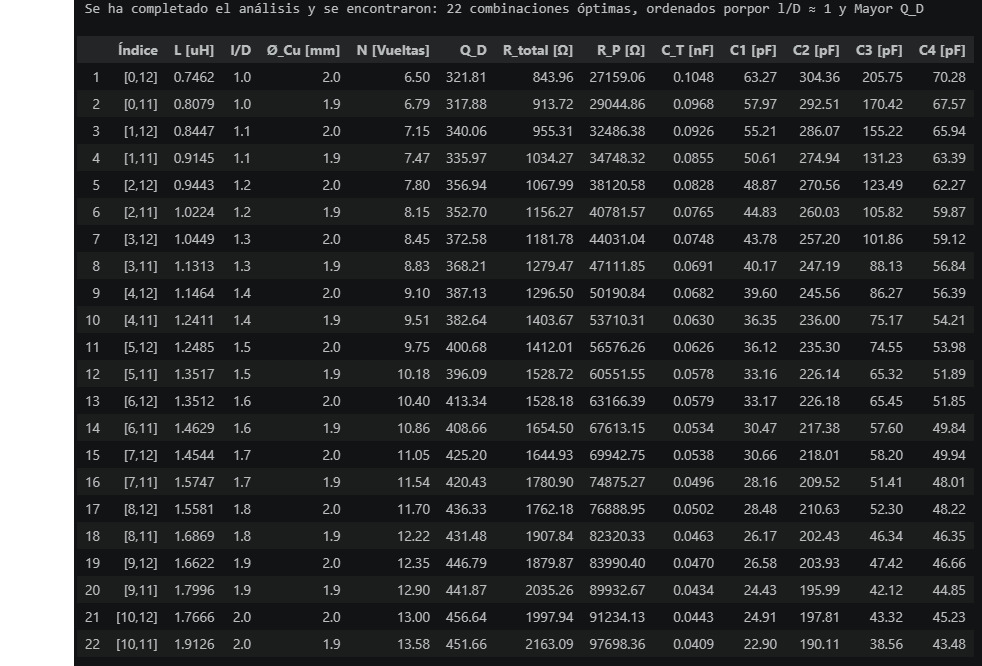
\includegraphics[width=1\linewidth]{Figura 5.png}
        \caption{Tabla de valores de $L$ y $C_{T}$ que satisfacen las restricciones impuestas.}
        \label{fig:fig_5}
    \end{figure}    
    
    Si se observa la tabla, se ve que se han calculado los valores de las capacitancias $C_{1}$, $C_{2}$, $C_{3}$ y $C_{4}$ lo cual no se ha explicado hasta ahora. Para demostrar como obtener tales capacitancias, se procede a realizar una simple demostración matemática. Esta demostración se caracteriza por que al demostrar los valores de los capacitores del puerto de entrada, el análisis resulta prácticamente el mismo para los capacitores del puerto de salida. Se propuso entonces despejar el valor de $C_{2}$ de \eqref{eq_7}, de modo que:
    \begin{equation}
        R_{G}' = R_{G} \left(1 + \frac{C_{2}}{C_{1}}\right)^{2}
        \label{eq_21}
    \end{equation}
    \begin{equation}
        \sqrt{\frac{R_{G}'}{R_{G}}} = 1 + \frac{C_{2}}{C_{1}}
        \label{eq_22}
    \end{equation}
    \begin{equation}
        C_{2} = C_{1} \left(\sqrt{\frac{R_{G}'}{R_{G}}} - 1\right)
        \label{eq_23}
    \end{equation}
    Reemplazando lo obtenido en \eqref{eq_23} en \eqref{eq_3}, se tiene que:
    \begin{equation}
        \frac{C_{T}}{2} = \frac{C_{1} C_{1} \left(\sqrt{\frac{R_{G}'}{R_{G}}} - 1\right)}{C_{1} + C_{1} \left(\sqrt{\frac{R_{G}'}{R_{G}}} - 1\right)}
        \label{eq_24}
    \end{equation}
    \begin{equation}
        \frac{C_{T}}{2} = \frac{C_{1} \left(\sqrt{\frac{R_{G}'}{R_{G}}} - 1\right)}{1 + \sqrt{\frac{R_{G}'}{R_{G}}} - 1}
        \label{eq_25}
    \end{equation}
    \begin{equation}
        C_{1}\left(\sqrt{\frac{R_{G}'}{R_{G}}} - 1\right) = \frac{C_{T}}{2}\sqrt{\frac{R_{G}'}{R_{G}}}
        \label{eq_26}
    \end{equation}
    Se sabe que el operando izquierdo de \eqref{eq_26} se corresponde con la expresión de $C_{2}$ definida en \eqref{eq_23}, tal que:
    \begin{equation}
        C_{2} = \frac{C_{T}}{2}\sqrt{\frac{R_{G}'}{R_{G}}}
        \label{eq_27}
    \end{equation}
    Luego, si se sigue operando sobre \eqref{eq_25}, se pudo despejar a $C_{1}$:
    \begin{equation}
        C_{1} = \frac{\frac{C_{T}}{2}\sqrt{\frac{R_{G}'}{R_{G}}}}{\sqrt{\frac{R_{G}'}{R_{G}}} - 1} = \frac{C_{2}}{\sqrt{\frac{R_{G}'}{R_{G}}} - 1}
        \label{eq_28}
    \end{equation}
    Como se mencionó inicialmente, se tiene que esta demostración es prácticamente la misma para el puerto de salida, de modo que operando sobre \eqref{eq_8} y \eqref{eq_4}, se deduce que:
    \begin{equation}
        C_{3} = \frac{C_{4}}{\sqrt{\frac{R_{L}'}{R_{L}}} - 1}
        \label{eq_29}
    \end{equation}
    \begin{equation}
        C_{4} = \frac{C_{T}}{2}\sqrt{\frac{R_{L}'}{R_{L}}}
        \label{eq_30}
    \end{equation}
    

    \item \underline{Paso 11:} Como paso final en el diseño del inductor y la capacitancia, se eligió manualmente el primer par inductor-capacitores ya que presentó las mejores condiciones tanto constructivas para el diseño del inductor, como para elegir los capacitores.
    En este paso, se ajustaron las capacidades a valores comerciales de acuerdo a los siguientes valores:
    \begin{itemize}
        \item $C_{1} = 47 + 15 = 62 \ [pF] \approx 63.27 \ [pF]$
        \item $C_{2} = 150 + 150 = 300 \ [pF] \approx 304.36 \ [pF]$
        \item $C_{3} = 180 + 22 = 202 \ [pF] \approx 205.75 [pF]$
        \item $C_{4} = 47 + 22 = 69 \ [pF] \approx 70.28 \ [pF]$
    \end{itemize}
    Nótese que tal ajuste de capacitancia, debe ser compensando por un ajuste en la inductancia para mantener la misma frecuencia de resonancia $f_{0}$. Esto implicó recalcular la inductancia y consecuentemente algunos parámetros constructivos del mismo, y para ello se tuvieron que establecer algunos criterios mínimos de que parámetros se podían ajustar, tales como:
    \begin{itemize}
        \item El número de espiras ($N$).
        \item El largo del inductor ($l$).
    \end{itemize}
    Y cuales parámetros no se debían ajustar:
    \begin{itemize}
        \item La separación entre espiras ($S = d_{C}$).
        \item El diámetro del cobre esmaltado ($d_{C} = 2 [mm]$).
    \end{itemize}
    Finalmente se obtuvieron los siguientes valores de inductancia y parámetros constructivos:

    \begin{figure}[htbp]
        \centering
        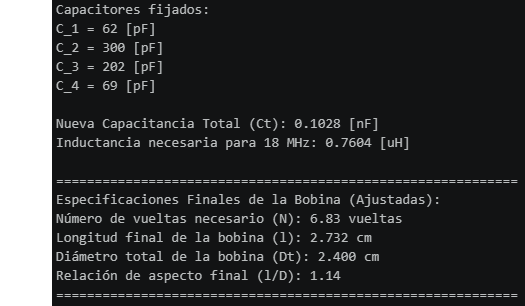
\includegraphics[width=0.95\linewidth]{Figura 6.png}
        \caption{Gráficas de interés para el diseño del inductor.}
        \label{fig:fig_6}
    \end{figure}
\end{itemize}



\subsection{Simulación en LTSpice}
Una vez concluidos los cálculos de diseño tanto del inductor como de los capacitores, se procedió a realizar una simulación del circuito en LTSpice del siguiente circuito:

\begin{figure}[htbp]
    \centering
    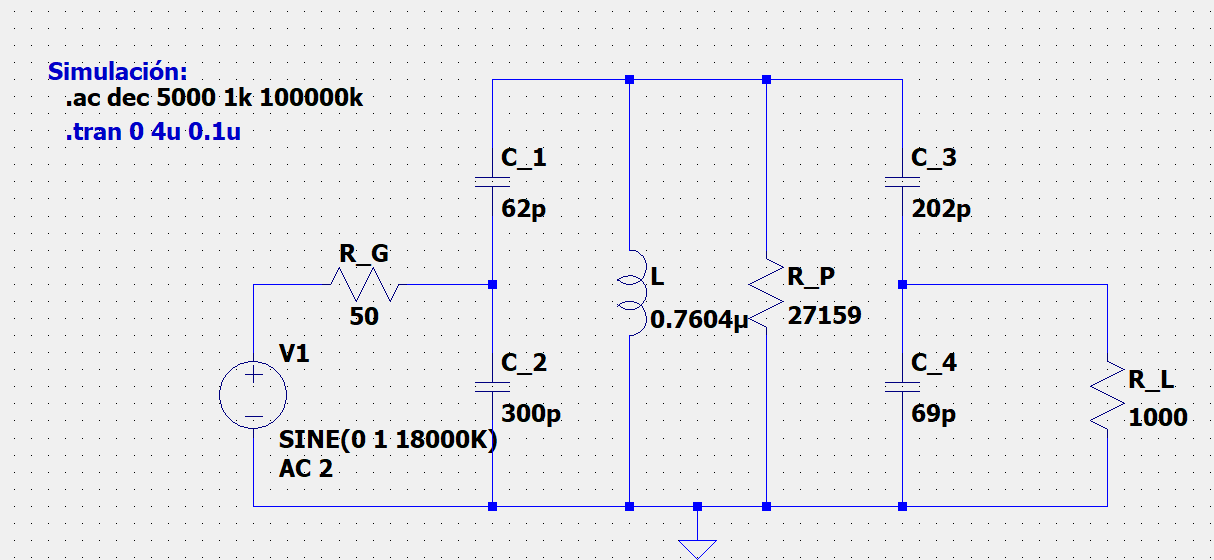
\includegraphics[width=1\linewidth]{Figura 7.png}
    \caption{Acoplador inter-etapa simulado en LTSpice.}
    \label{fig:fig_7}
\end{figure}

Una vez definido el circuito en base a los parámetros definidos en el final de la sección precedente a esta, se realizaron las siguientes mediciones:
\begin{itemize}
    \item \underline{Medición de $f_{0}$ y $BW$:} Para ello, se utilizó el circuito el circuito tal como se muestra en la Fig. \ref{fig:fig_7} y se realizó un barrido de señales de AC en frecuencia para obtener el diagrama de bode de módulo y fase. Para estas mediciones sólo importa el diagrama de módulo el cual se muestra en la Fig. \ref{fig:fig_8}.

    \begin{figure}[htbp]
        \centering
        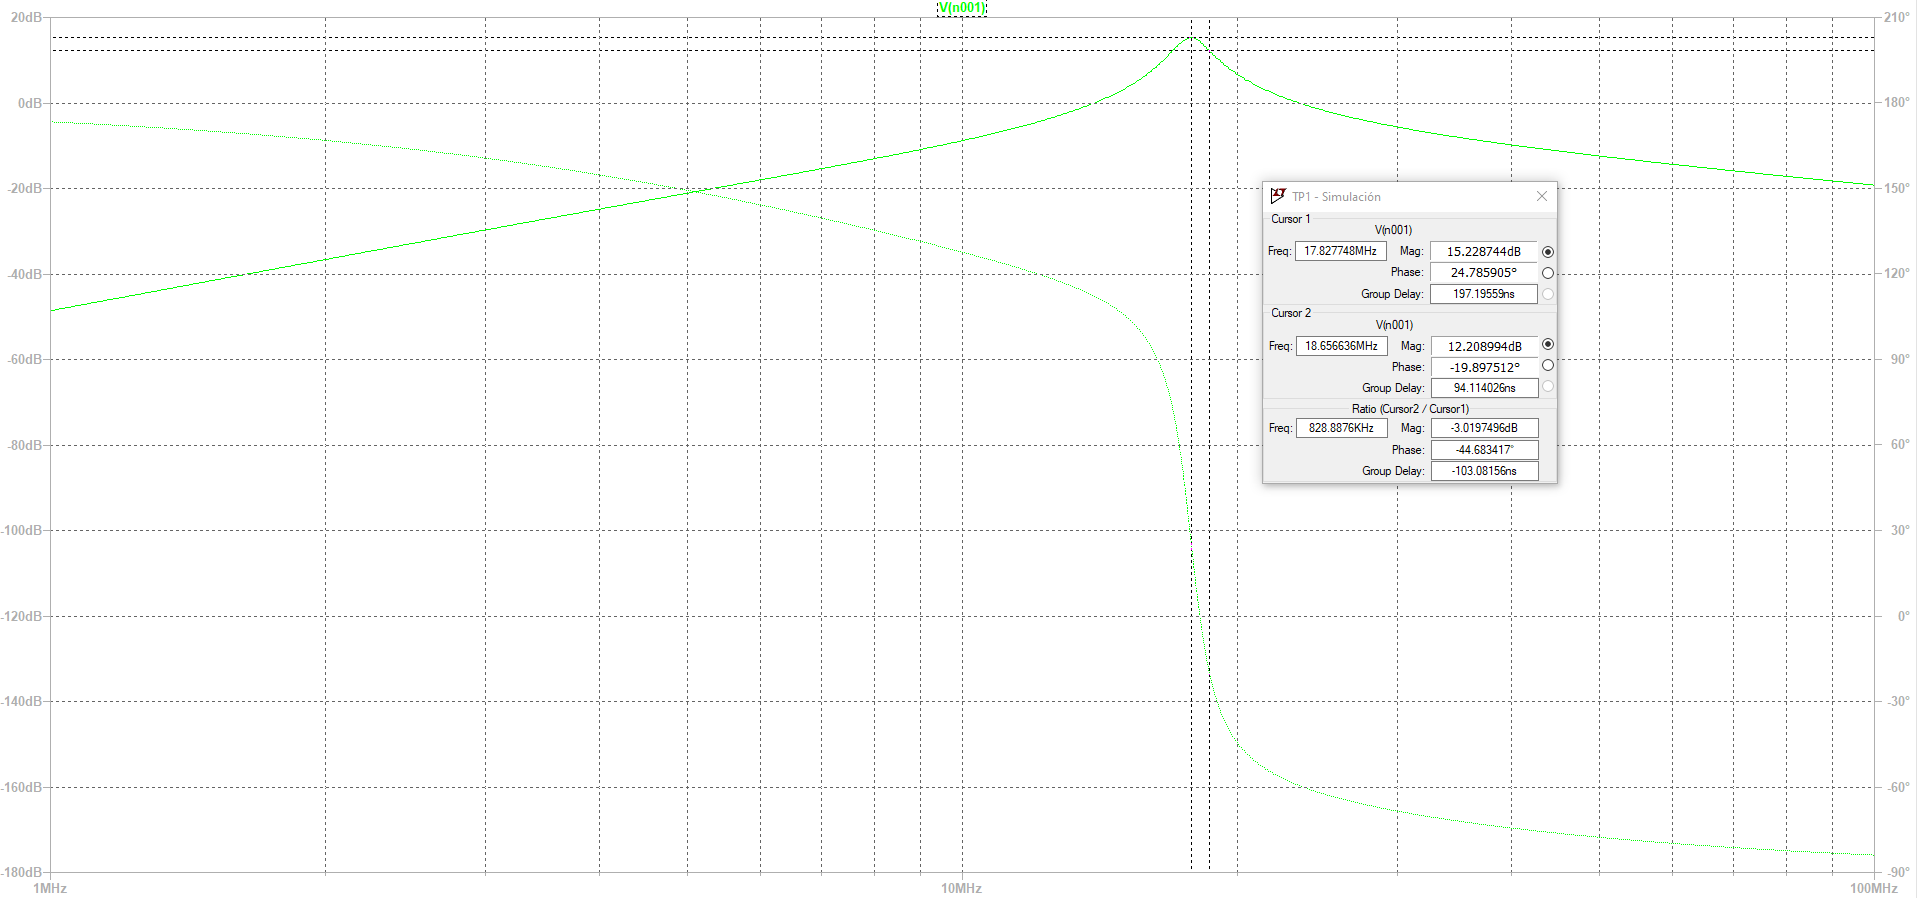
\includegraphics[width=0.95\linewidth]{Figura 8.png}
        \caption{Medición de $f_{0}$ y $BW$ en LTSpice.}
        \label{fig:fig_8}
    \end{figure}

    Observando los valores que entrega el simulador de la Fig. \ref{fig:fig_8}, se tiene que:
    \begin{itemize}
        \item $f_{0} \approx 17.82 \ [MHz]$
        \item $BW = 2(828.88 \ [kHz]) \approx 1.65 \ [MHz]$
    \end{itemize}

    Se obtiene de aquí un $Q_{C} = \frac{17.82}{1.65} \approx 10.8$. \\

    \item \underline{Medición de $Z_{in}$}: Para ello, se sabe que si el circuito está en la frecuencia de resonancia, se tiene que la caída de tensión luego de $R_{G}$ debe ser igual a la mitad del valor de la fuente, ya que la impedancia que ve el circuito hacia el otro lado deberá ser la misma.
    Realizando una simulación transitoria de señal a la frecuencia de resonancia, se obtuvieron las formas de onda descritas en Fig. \ref{fig:fig_9}.

    \begin{figure}[htbp]
        \centering
        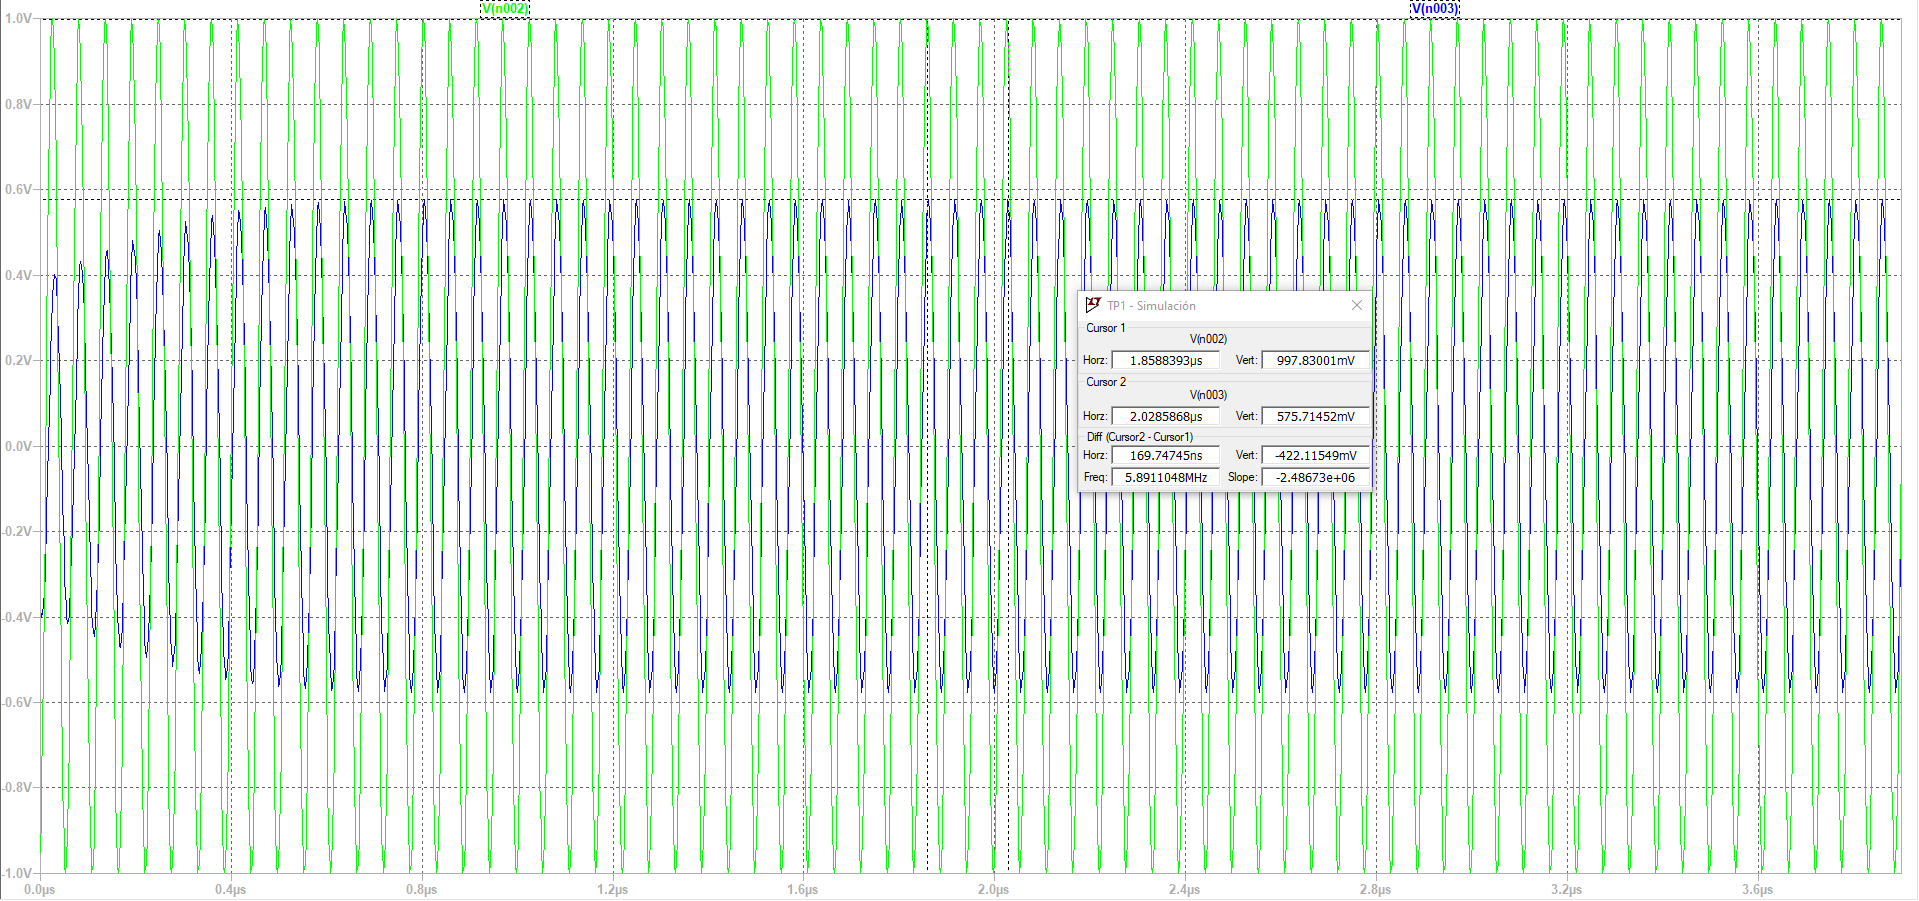
\includegraphics[width=0.95\linewidth]{Figura 9.png}
        \caption{Medición de $Z_{in}$ en LTSpice.}
        \label{fig:fig_9}
    \end{figure}

    Se tuvo que la tensión de la fuente es igual a: $V_{G} = 1 \ [V]$ y la caída de tensión luego de $R_{G}$ es de: $0.575 \ [V]$. Nótese que la caída de tensión no dió exactamente $\frac{V_{G}}{2}$, sino un valor un poco mayor, lo que indica que hay cierta des-adaptación en la entrada. Para calcularla, se planteó el circuito equivalente de la Fig. \ref{fig:fig_10}
    
    \begin{figure}[htbp]
        \centering
        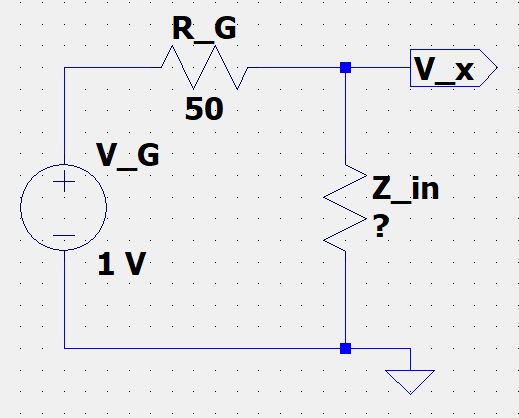
\includegraphics[width=0.5\linewidth]{Figura 10.png}
        \caption{Divisor resistivo a la entrada.}
        \label{fig:fig_10}
    \end{figure}

    Vemos que se trata de un simple divisor resistivo, donde la única incógnita es $Z_{in}$, por lo tanto:
    \begin{equation}
        V_{x} = \frac{V_{in}}{R_{G} + Z_{in}}(Z_{in})
        \label{eq_31}
    \end{equation}
    \begin{equation}
        V_{x}(R_{G} + Z_{in}) = V_{in}(Z_{in})
        \label{eq_32}
    \end{equation}
    \begin{equation}
        V_{x}(R_{G}) = Z_{in}(V_{in} - V_{x})
        \label{eq_33}
    \end{equation}
    \begin{equation}
        Z_{in} = \frac{V_{x}(R_{G})}{V_{in} - V_{x}}
        \label{eq_34}
    \end{equation}
    Reemplazando por lo obtenido en la simulación, se deduce que:
    \begin{equation}
        Z_{in} = \frac{0.575(50)}{1 - 0.575} \approx 67.64 \ [\Omega]
        \label{eq_35}
    \end{equation} \\

    \item \underline{Medición de $Z_{out}$:} El concepto fundamental para esta medición es el mismo que el que se utilizó para medir $Z_{in}$: Se medió la tensión de salida del circuito con $R_{L}$ desconectada y luego se medió la misma salida con $R_{L}$ conectada. Es de esperarse que en la frecuencia de resonancia, la tensión de salida caiga a la mitad al conectar la carga. Se presenta en la Fig. \ref{fig:fig_12} y Fig. \ref{fig:fig_11} las tensiones de salida con y sin $R_{L}$ respectivamente.

    \begin{figure}[htbp]
        \centering
        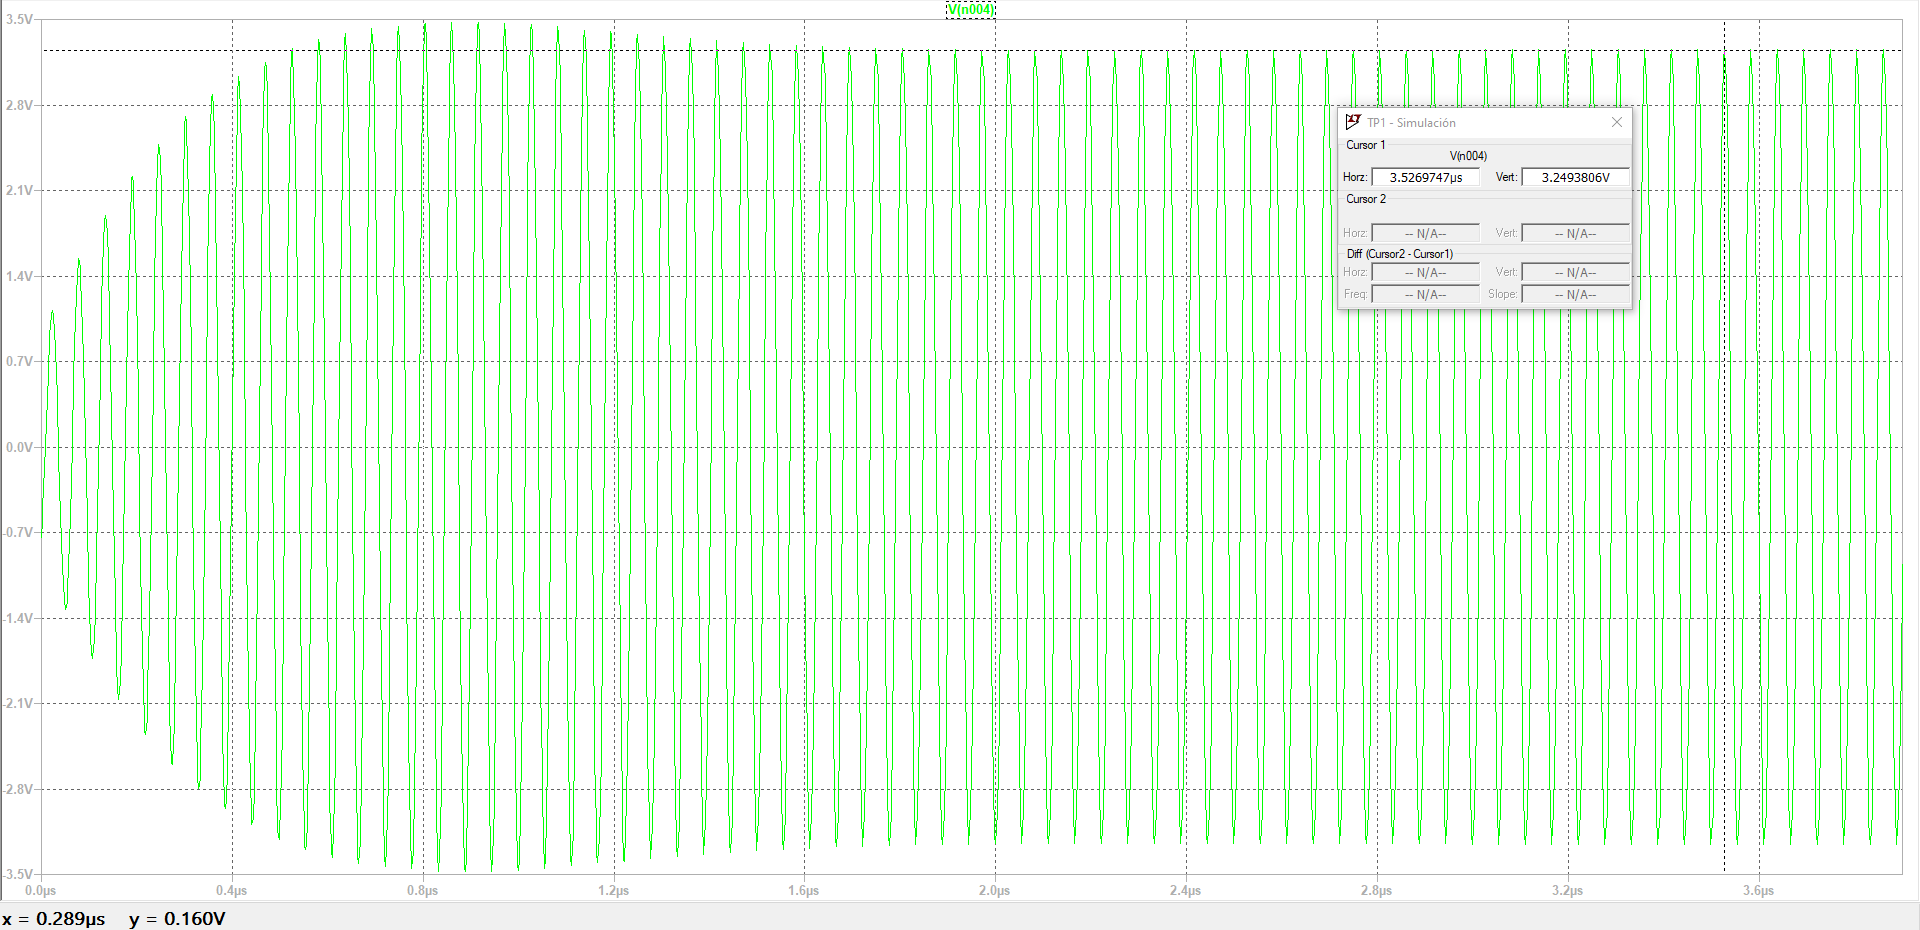
\includegraphics[width=0.95\linewidth]{Figura 11.png}
        \caption{Medición de $Z_{out}$ sin $R_{L}$ en LTSpice.}
        \label{fig:fig_11}
    \end{figure}

    \begin{figure}[htbp]
        \centering
        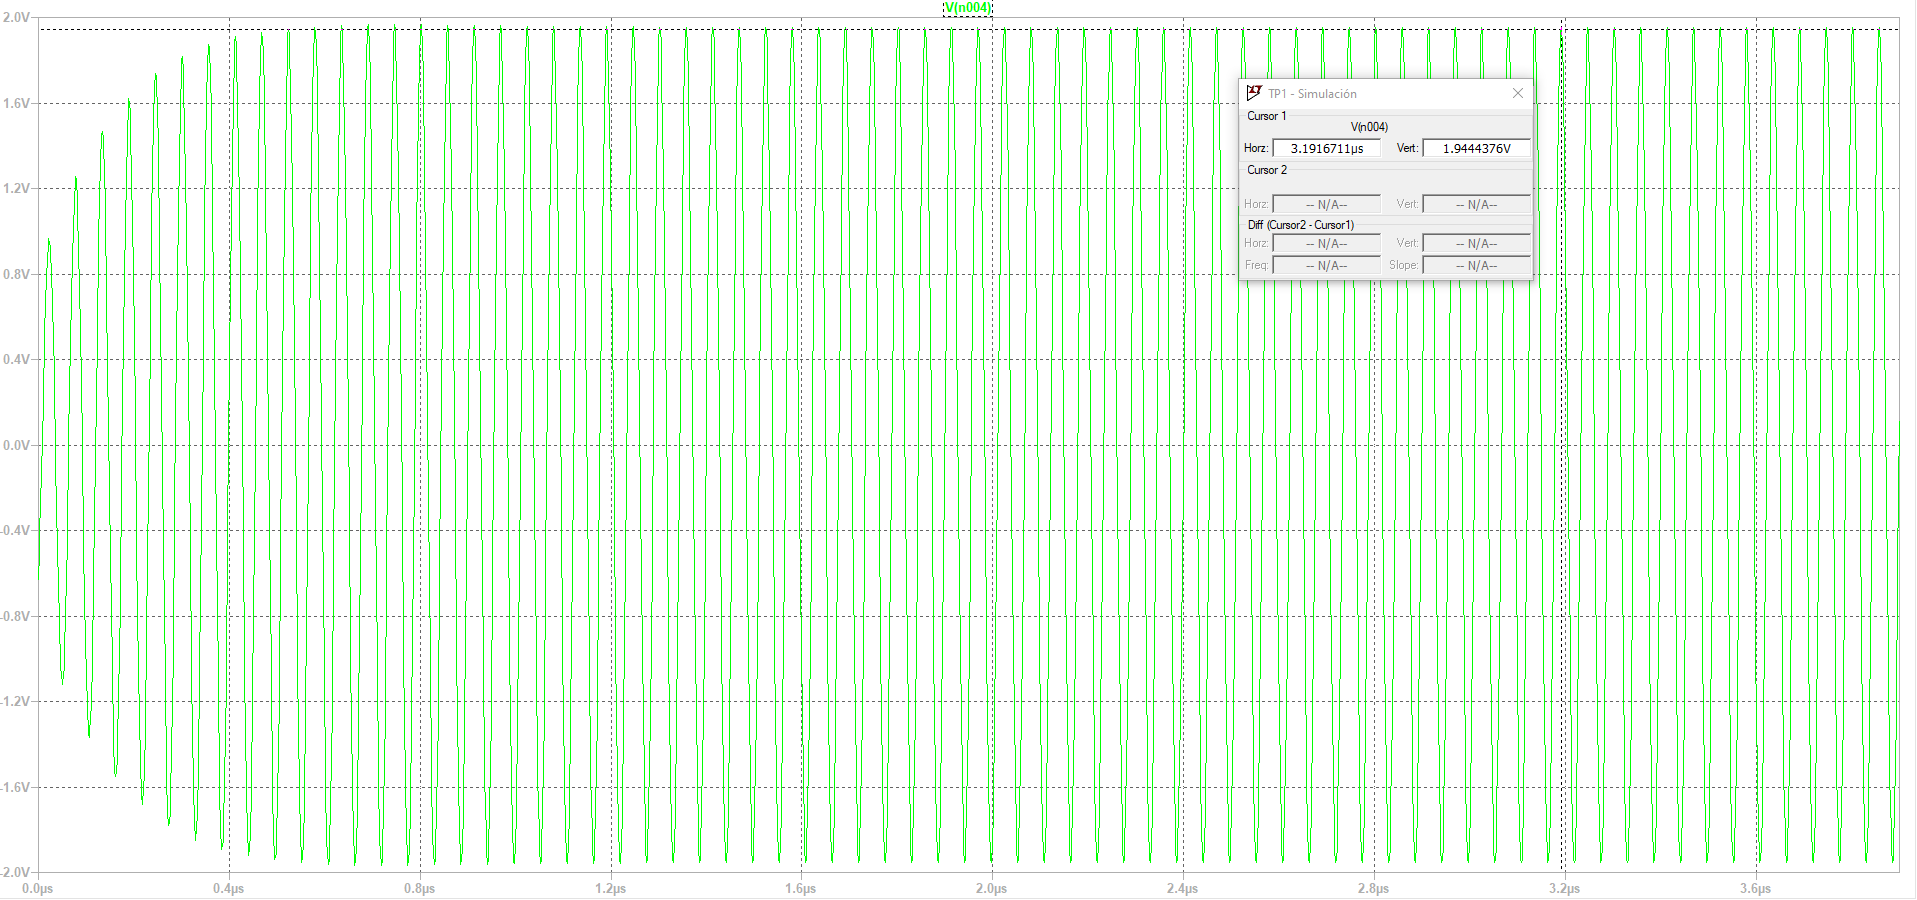
\includegraphics[width=0.95\linewidth]{Figura 12.png}
        \caption{Medición de $Z_{out}$ con $R_{L}$ en LTSpice.}
        \label{fig:fig_12}
    \end{figure}

    Vemos que la caída de tensión sin $R_{L}$, es de: $V_{0(NL)} \approx 3.24 \ [V] $ pero cuando se conecta $R_{L}$, esta caída de tensión es de: $1.94 \ [V]$. Nuevamente, se pudo determinar la des-adaptación mediante un simple divisor resistivo tal como el que se muestra en la Fig \ref{fig:fig_13}.

    \begin{figure}[htbp]
        \centering
        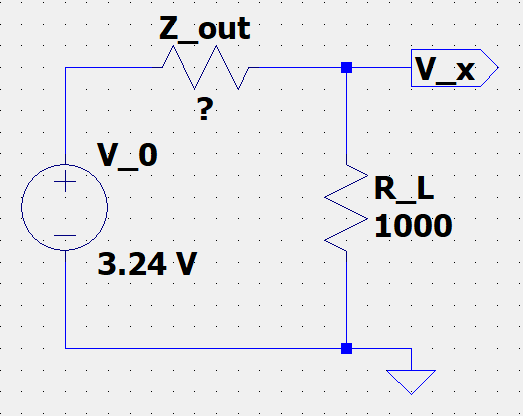
\includegraphics[width=0.5\linewidth]{Figura 13.png}
        \caption{Divisor resistivo a la salida.}
        \label{fig:fig_13}
    \end{figure}

    En este divisor resistivo, se tienen que todos los valores son datos exceptuando a $Z_{out}$, tal que planteando la ecuación del divisor:
    \begin{equation}
        V_{x} = \frac{V_{out}}{Z_{out} + R_{L}}(R_{L})
        \label{eq_36}
    \end{equation}
    \begin{equation}
        Z_{out} + R_{L} = \frac{V_{out}(R_{L})}{V_{x}}
        \label{eq_37}
    \end{equation}
    \begin{equation}
        Z_{out} = \frac{V_{out}(R_{L})}{V_{x}} - R_{L} 
        \label{eq_38}
    \end{equation}
    Reemplazando por lo obtenido en la simulación, se deduce que:
    \begin{equation}
            Z_{out} = \frac{3.24(1000)}{1.94} - 1000 \approx 670.1 \ [\Omega]
        \label{eq_39}
    \end{equation}
\end{itemize}



\subsection{Armado y Mediciones Físicas del Circuito}
Si bien se realizó un análisis posterior a esta sección sobre los resultados obtenidos, es posible decir que los valores de simulación del circuito fueron relativamente próximos a los valores de diseño del acoplador, por lo tanto se decidió realizar el armado físico del circuito el cual se presenta en la Fig. \ref{fig:fig_14}.

\begin{figure}[htbp]
    \centering
    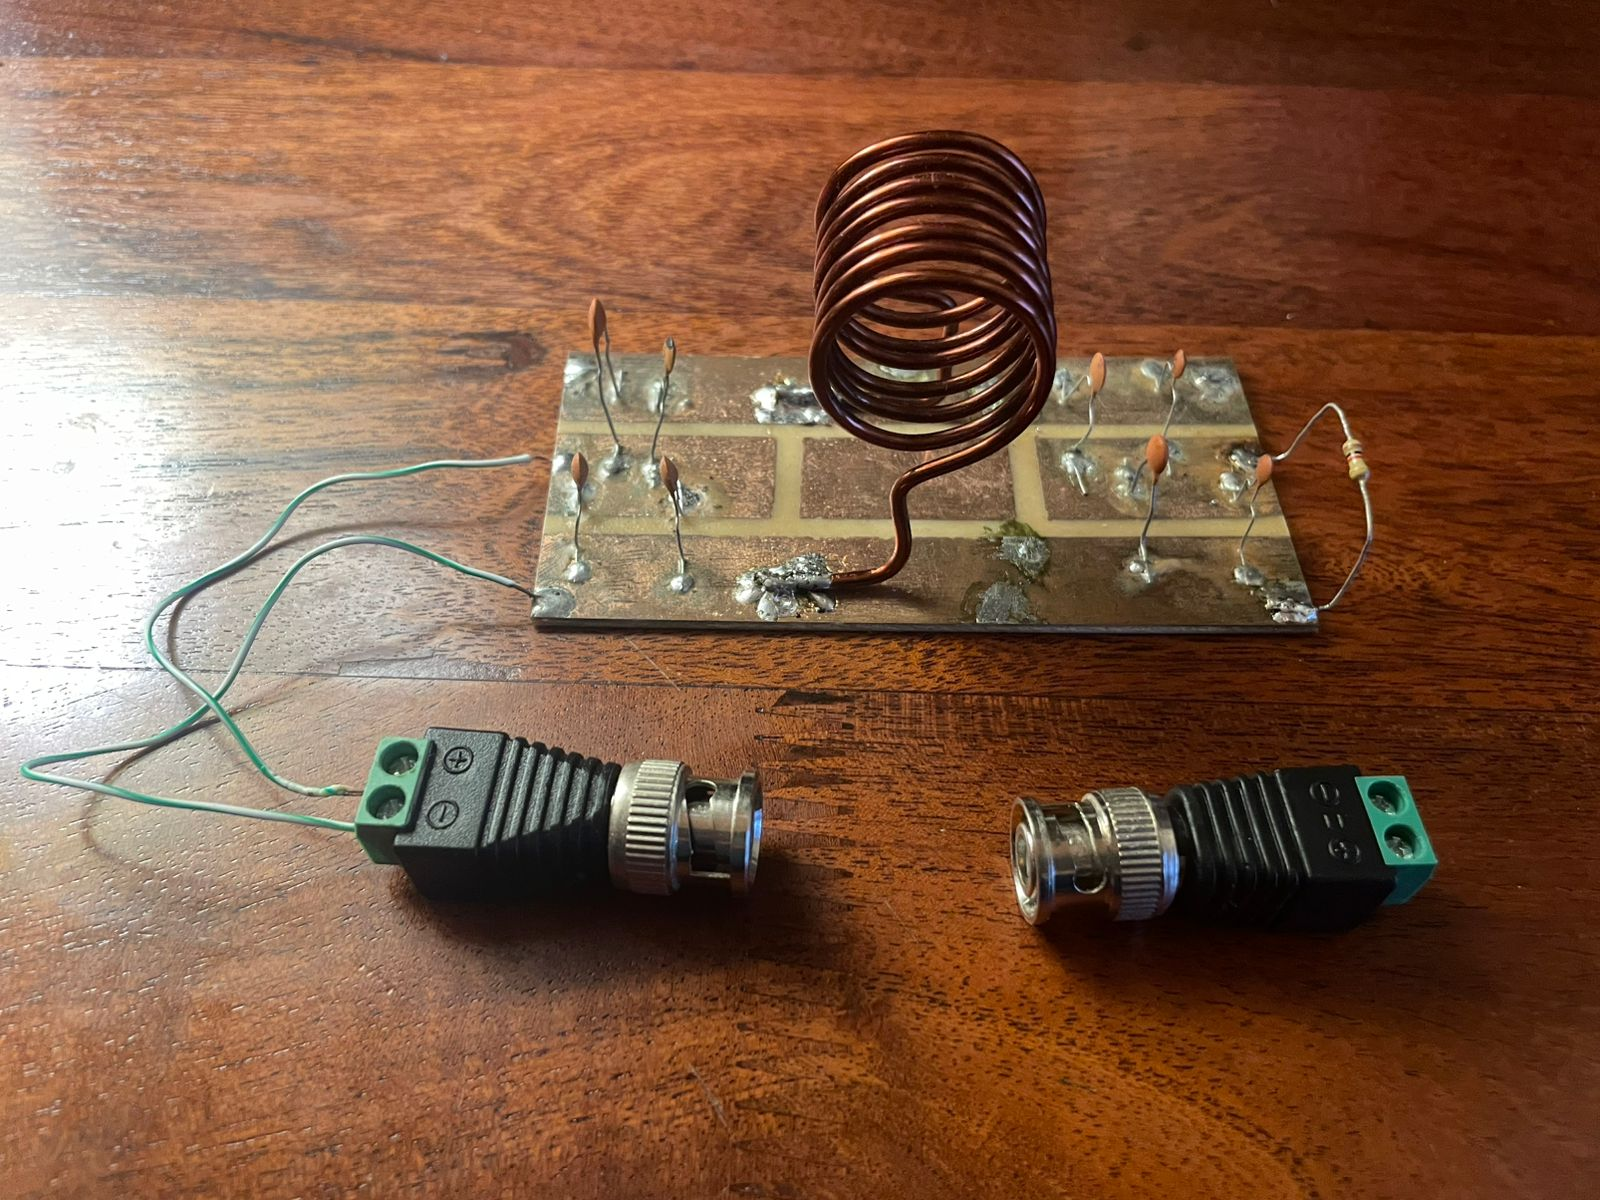
\includegraphics[width=0.8\linewidth]{Figura 14.png}
    \caption{Armado físico del circuito.}
    \label{fig:fig_14}
\end{figure}

Antes de comenzar con el análisis de las mediciones físicas, hay ciertos aspectos constructivos del circuito que deben ser mencionados:
\begin{itemize}
    \item Si bien se realizaron los cálculos y diseño del inductor para un diámetro de cobre esmaltado de: $d_{C} = 0.2 \ [cm]$, se tiene que el inductor fue armado con un diámetro de cobre de: $d_{C} = 0.195 \ [cm]$. Si bien parece una diferencia insignificante, se tiene que una variación en el diámetro del cobre esmaltado, indudablemente afectó al valor de la inductancia.
    
    \item También deben realizarse ciertas consideraciones constructivas del inductor: Una de ellas siendo el número de espiras ($N$). Si bien en la Fig. \ref{fig:fig_6} se concluyó que el numero de vueltas debería ser de $6.83 \ [vueltas]$, se tuvo que redondear este valor a $7 \ [vueltas]$ debido a la imposibilidad constructiva de realizar un número no entero de vueltas. Al igual que para la consideración anterior, modificar el número de espiras, indudablemente afectó al valor de la inductancia.
    
    \item Para evitar el uso de cables BNC-Cocodrilo, se optó por utilizar los adaptadores BNC-Macho a Hembra que se observan en la Fig. \ref{fig:fig_14}. Esto se realizó con el fin de evitar que las capacidades parásitas generadas por los cables cocodrilos interfieran en las mediciones físicas del circuito, dado que en una frecuencia de trabajo de $f_{0} = 18 \ [MHz]$, resultan en impedancias considerables a las mediciones.
\end{itemize}

Con estas consideraciones en mente, se procedió con la medición de valores de interés del circuito:
\begin{itemize}
    \item \underline{Medición de $f_{0}$:} La forma de conectar el circuito para medir la frecuencia de resonancia es la que se muestra en la Fig. \ref{fig:fig_15}. Allí, se buscó variar la frecuencia del generador hasta encontrar un pico de amplitud de la señal de entrada.

    \begin{figure}[htbp]
        \centering
        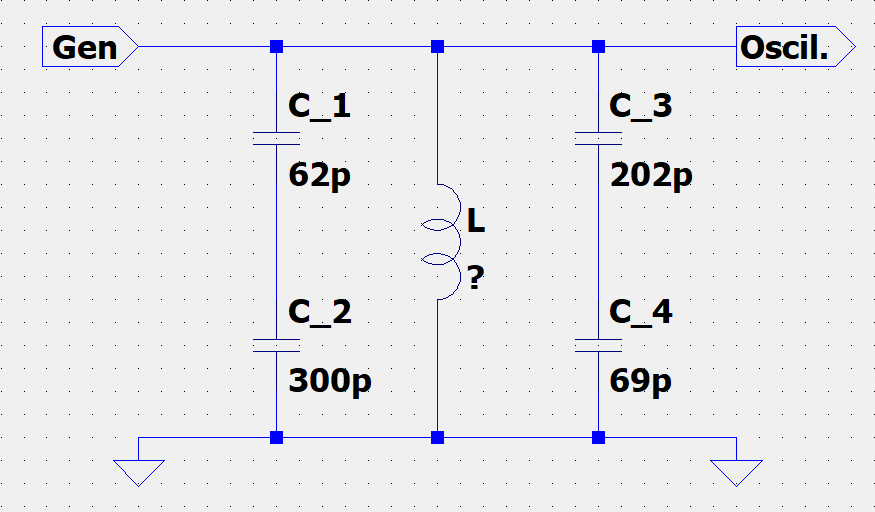
\includegraphics[width=0.7\linewidth]{Figura 15.png}
        \caption{Medición de $f_{0}$.}
        \label{fig:fig_15}
    \end{figure}

    Nótese que en la práctica, la introducción de cualquier elemento de medición tendrá como consecuencia la introducción de la capacidad parásita interna del mismo, lo cual afectará consecuentemente a la medición y por lo tanto nunca se medirá $f_{0}$ directamente, sino más bien se mide:
    \begin{equation}
        f_{0}' = \frac{1}{2\pi\sqrt{LC_{M}}}
        \label{eq_40}
    \end{equation}
    Se tiene que esta frecuencia no toma en cuenta solo las capacidades utilizadas en el circuito físico, sino también las capacidades parásitas del osciloscopio, del generador, de los cables, etcétera. 
    Nótese además que en \eqref{eq_40}, se tiene una ecuación con 2 incógnitas: $L$ y $C_{M}$ ya que si bien se puede medir $f_{0}'$ siguiendo el conexionado de la Fig. \ref{fig:fig_15}, no se conoce el valor de la inductancia armada la cual, como se mencionó en las consideraciones, puede ser distinto al valor de diseño.
    Para resolver este inconveniente, lo que se hizo fue introducir un capacitor comercial de valor $C_{x}$ conocido, en paralelo con la inductancia. De esta forma, lo que se logra es generar una nueva frecuencia de resonancia denominada $f_{0}''$ la cual se definió como:
    \begin{equation}
        f_{0}'' = \frac{1}{2\pi\sqrt{L(C_{M} + C_{x})}}
        \label{eq_41}
    \end{equation}
    Nótese que entre \eqref{eq_40} y \eqref{eq_41}, se tiene un sistema de 2 ecuaciones y 2 incógnitas, de modo tal que se tiene una solución única para $L$ y $C_{M}$. Para resolver este sistema se propuso elevar a \eqref{eq_40} y a \eqref{eq_41} al cuadrado y luego plantear la división entre ambas, es decir:
    \begin{equation}
        \left(\frac{f_{0}'}{f_{0}''}\right)^{2} = \frac{\frac{1}{4\pi^{2} L C_{M}}}{\frac{1}{4\pi^2 L (C_{M} + C_{x})}}
        \label{eq_42}
    \end{equation}
    Simplificando términos comunes:
    \begin{equation}
        \left(\frac{f_{0}'}{f_{0}''}\right)^{2} = \frac{C_{M} + C_{x}}{C_{M}} = 1 + \frac{C_{x}}{C_{M}}
        \label{eq_43}
    \end{equation}
    \begin{equation}
        C_{M} = \frac{C_{x}}{\left(\frac{f_{0}'}{f_{0}''}\right)^{2} - 1}
        \label{eq_44}
    \end{equation}
    Luego se tiene que sabiendo el valor de $C_{M}$, se puede despejar a $L$ como:
    \begin{equation}
        L = \frac{1}{(2\pi f_{0}')^{2} C_{M}}
        \label{eq_45}
    \end{equation}
    Finalmente, se tiene que sabiendo el valor de $L$ y $C_{T}$, se pudo calcular a $f_{0}$ siguiendo \eqref{eq_1}. Para realizar la medición, se utilizó un $C_{x} = 120 \ [pF]$ y se midió que las amplitudes máximas se encontraban en:
    \begin{itemize}
        \item $f_{0}' \approx 15.65 \ [MHz]$
        \item $f_{0}'' \approx 11.4 \ [MHz]$
    \end{itemize}
    De aquí se dedujo que según \eqref{eq_44}, la capacidad $C_{M}$ es:
    \begin{equation}
        C_{M} = \frac{120x10^{-12}}{\left(\frac{15.65}{11.4}\right)^{2} - 1} \approx 135.65 \ [pF]
        \label{eq_46}
    \end{equation}
    Por lo tanto, la inductancia es, según \eqref{eq_45}, igual a:
    \begin{equation}
        L = \frac{1}{(2\pi15.65x10^{6})^{2}(135.65x10^{-12})}\approx 0.7623 \ [\mu Hy]
        \label{eq_47}
    \end{equation}
    Finalmente, se tiene que combinando a $L$ de \eqref{eq_47} y a $C_T = 102.8 \ [pF]$ de la Fig. \ref{fig:fig_6}, la frecuencia de resonancia fue igual a:
    \begin{equation}
        f_{0} = \frac{1}{2\pi\sqrt{(0.7623x10^{-6})(102.8x10^{-12})}} \approx 17.97 \ [MHz]
        \label{eq_48}
    \end{equation}

    \item \underline{Medición del $BW$:} Para medir el ancho de banda, simplemente se conectó el circuito tal cual se lo muestra en la Fig. \ref{fig:fig_7} donde se conectó el canal del osciloscopio a bornes de $R_{L}$. Luego se localizó la frecuencia de resonancia del circuito físico tal como muestra la Fig. \ref{fig:fig_16}.

    \begin{figure}[htbp]
        \centering
        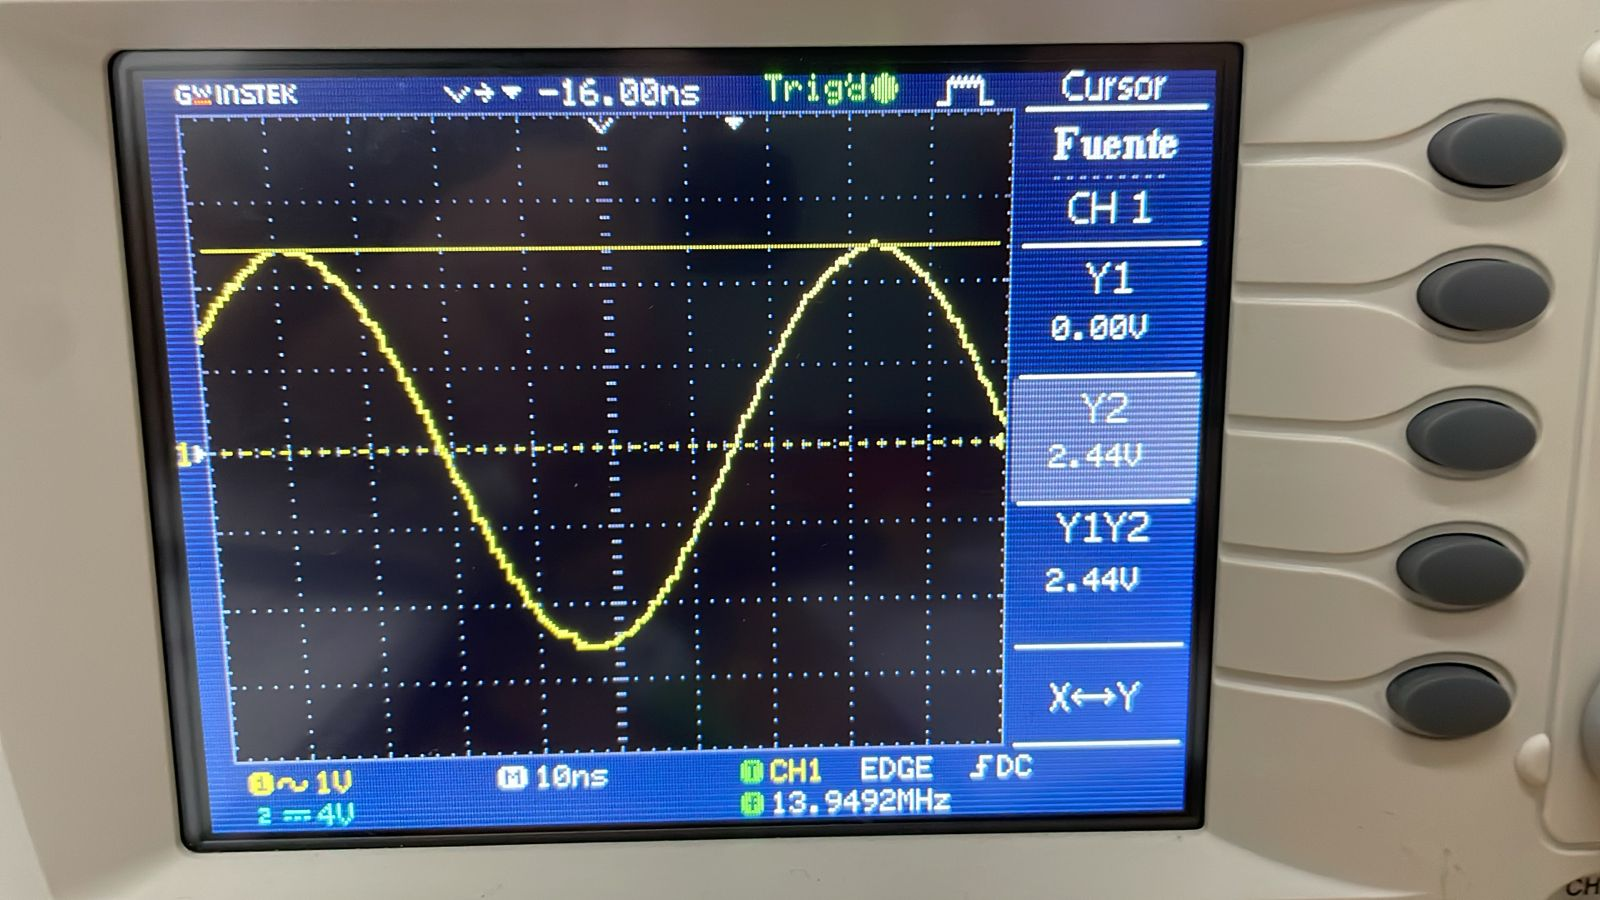
\includegraphics[width=0.8\linewidth]{Figura 16.jpeg}
        \caption{Medición de $BW$.}
        \label{fig:fig_16}
    \end{figure}

    Se observa aquí que la $f_0 = 13.95 \ [MHz]$ y la tensión a la salida es de: $V_{out} = 2.44 \ [V]$. Luego buscaremos la caída de $-3 \ [dB]$ en la tensión de salida, lo que equivale a que la tensión de salida sea igual a: $V_{out}' = 1.72 \ [V]$. Se identifican en la Fig. \ref{fig:fig_17} y en la Fig. \ref{fig:fig_18}, los límites inferiores y superiores respectivamente.
    
    \begin{figure}[htbp]
        \centering
        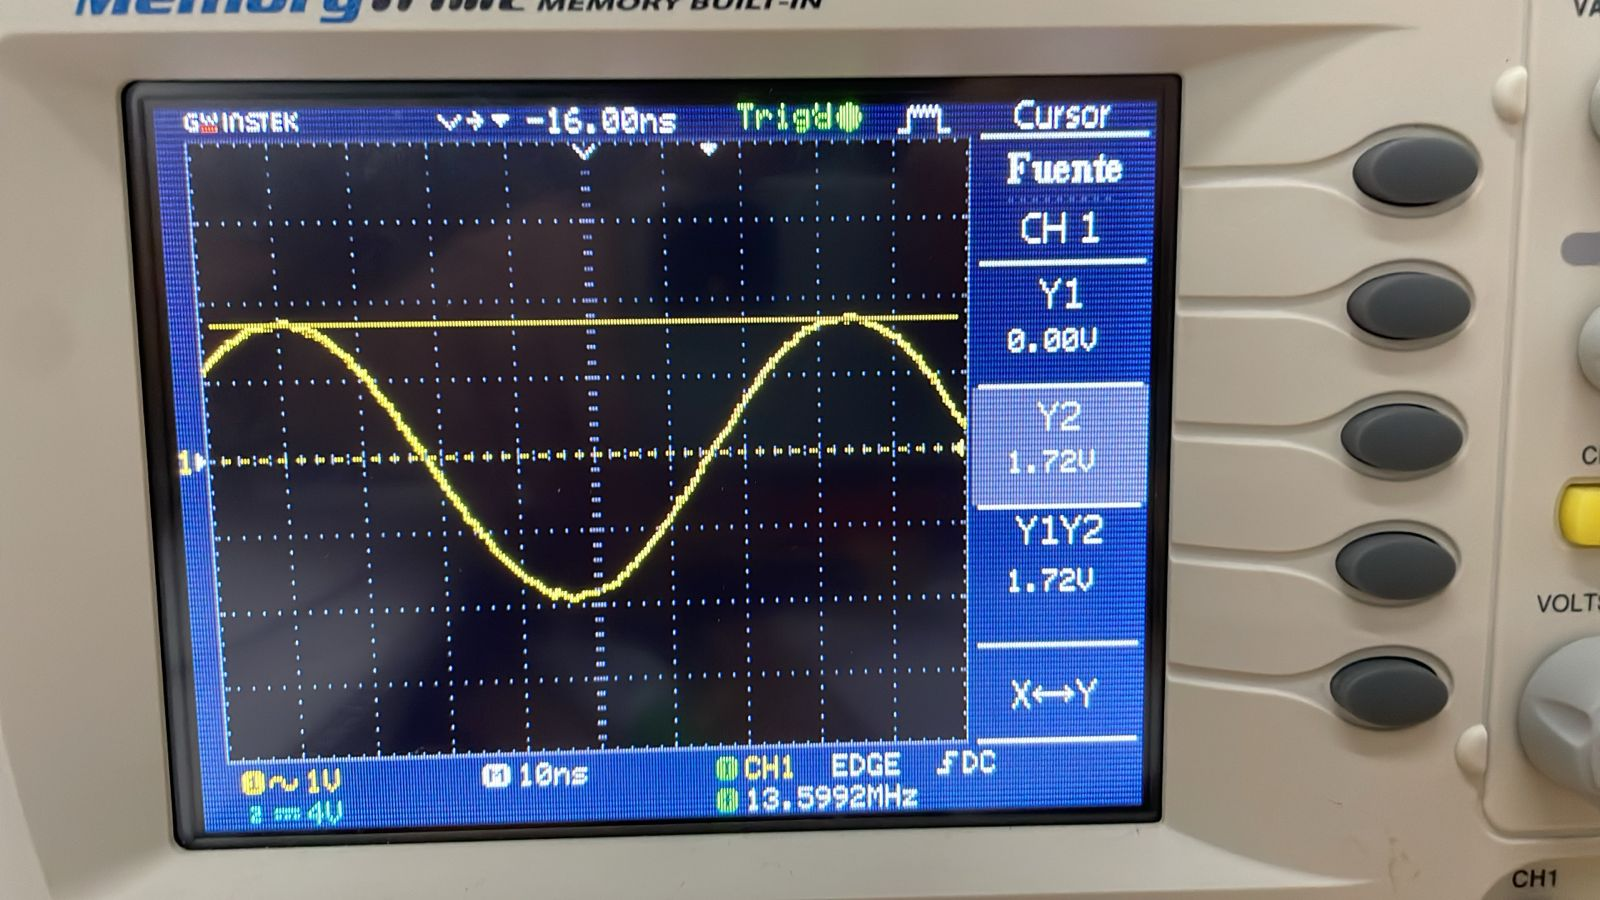
\includegraphics[width=0.8\linewidth]{Figura 17.jpeg}
        \caption{Medición del límite inferior del $BW$.}
        \label{fig:fig_17}
    \end{figure}

    \begin{figure}[htbp]
        \centering
        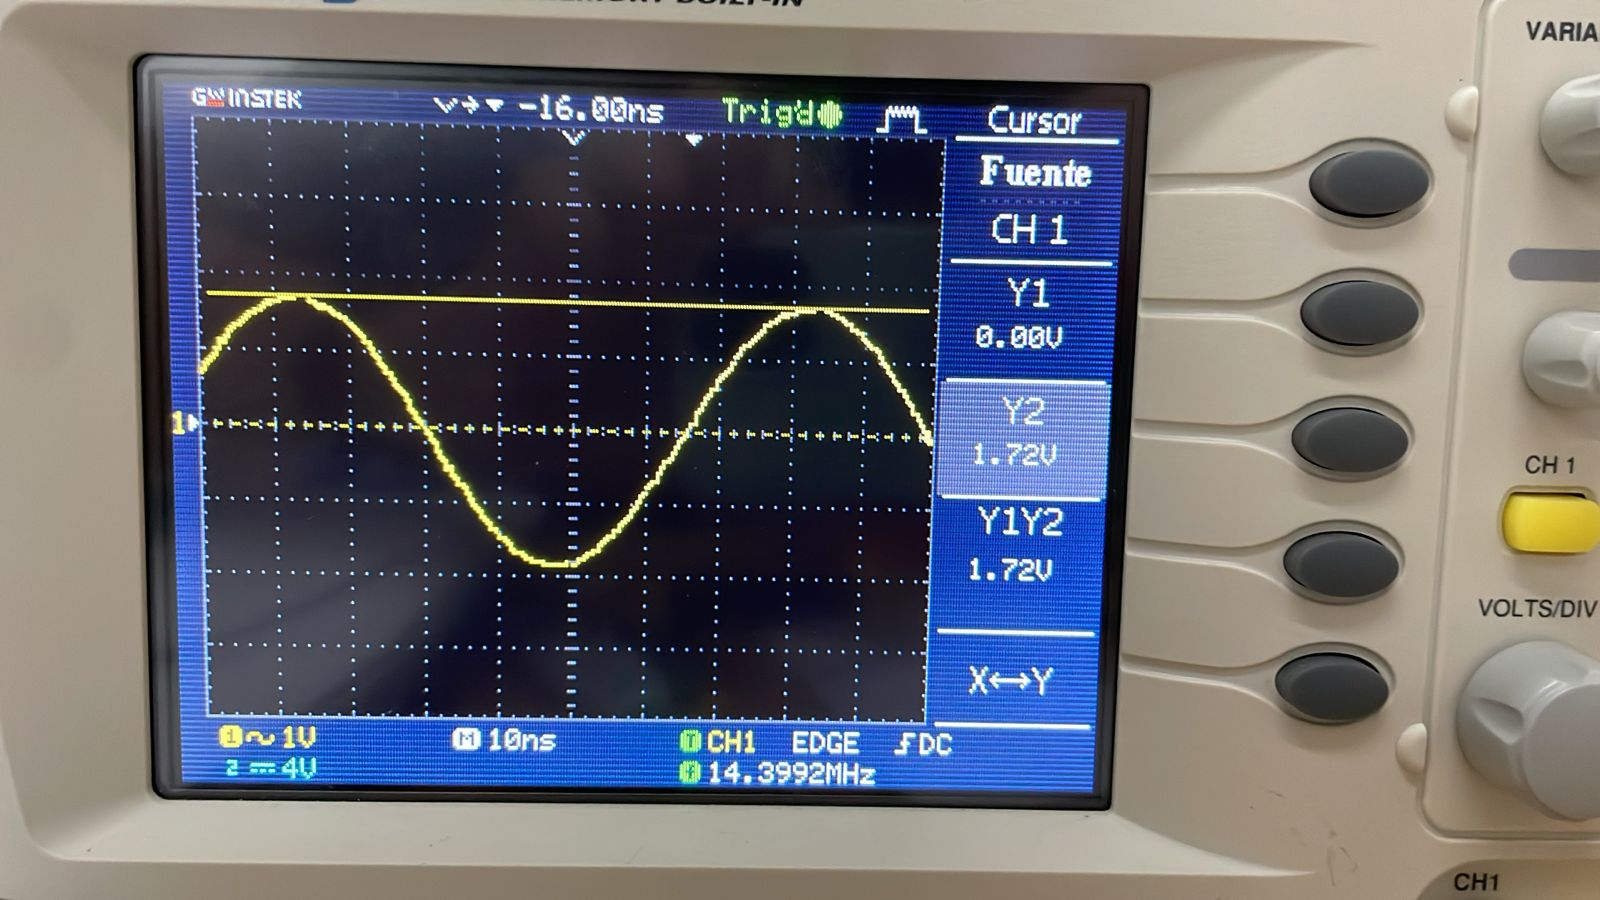
\includegraphics[width=0.8\linewidth]{Figura 18.jpeg}
        \caption{Medición del límite superior del $BW$.}
        \label{fig:fig_18}
    \end{figure}

    Se observa aquí que: $f_{min} = 13.6 \ [MHz]$ y que: $f_{max} = 14.4 \ [MHz]$, tal que el ancho de banda será igual a:
    \begin{equation}
        BW = 14.4 - 13.6 = 0.8 \ [MHz]
        \label{eq_49}
    \end{equation}
    Se puede calcular entonces el factor de calidad cargado según \eqref{eq_2} tal que:
    \begin{equation}
        Q_{C} = \frac{13.95}{0.8} \approx 17.43 \ [\%]
        \label{eq_50}
    \end{equation} \\

    \item \underline{Medición de $Z_{in}$:} Esta medición se realizó de la misma forma en la que se simuló la medición de la impedancia de entrada del circuito en LTSpice. Aquí se tiene que ajustando el circuito a su frecuencia de resonancia y con una $V_{G} = 1 \ [V]$, se observó en la Fig. \ref{fig:fig_19} una tensión del puerto de entrada al acoplador igual a: $V_{x} = 0.512 \ [V]$.

    \begin{figure}[htbp]
        \centering
        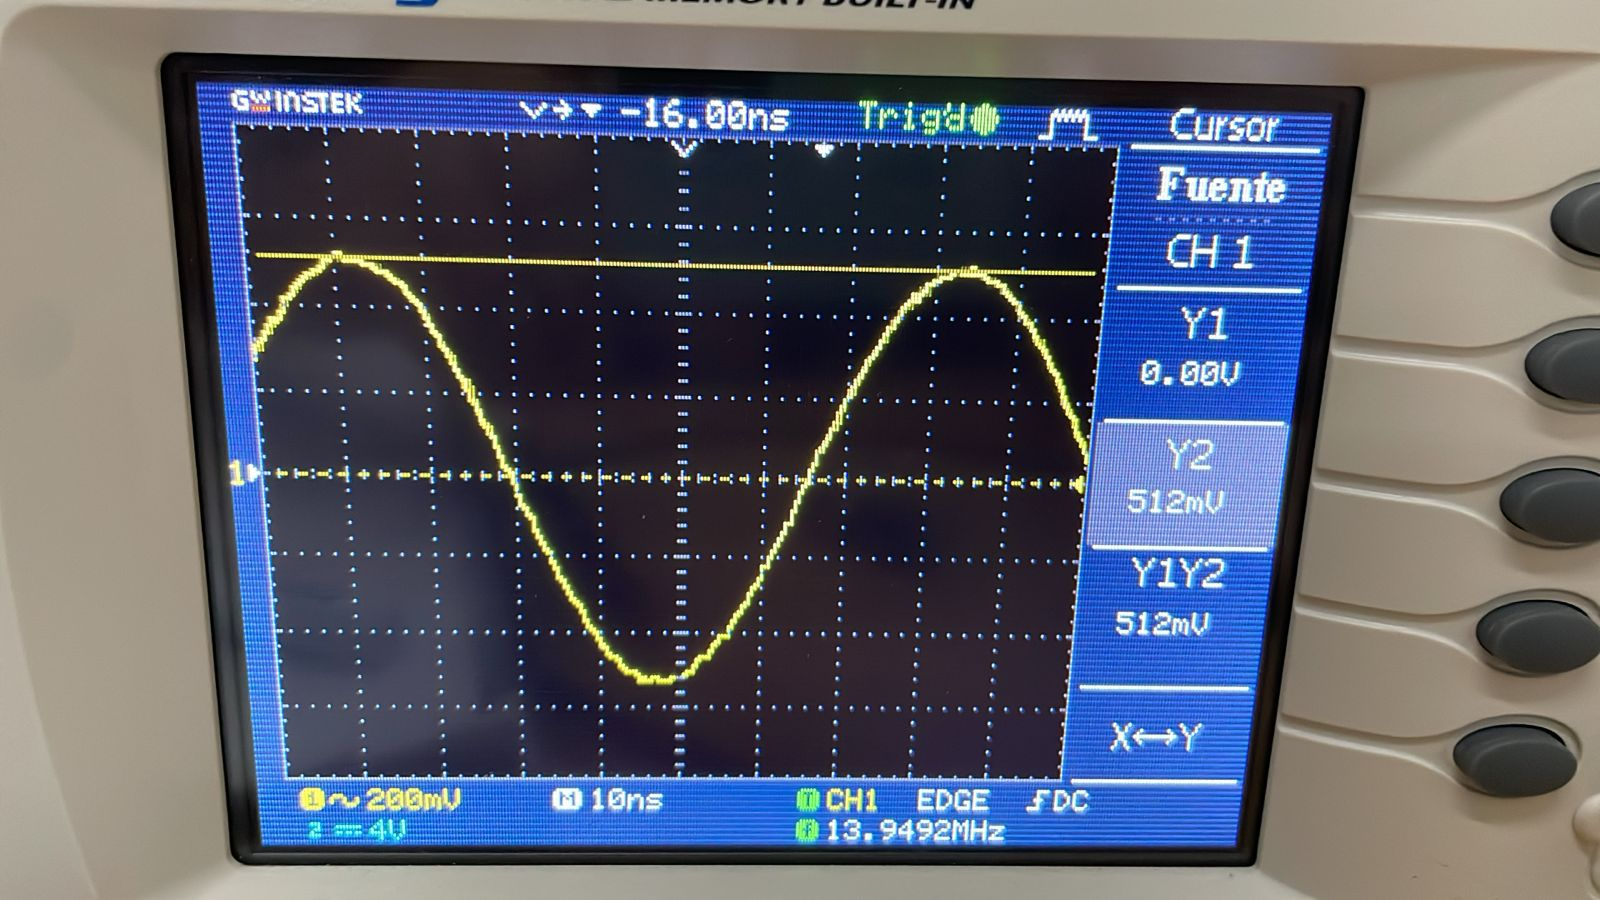
\includegraphics[width=0.8\linewidth]{Figura 19.jpeg}
        \caption{Medición de $Z_{in}$.}
        \label{fig:fig_19}
    \end{figure}
    
    Aplicando \eqref{eq_34}, se tiene que:
    \begin{equation}
        Z_{in} = \frac{0.512(50)}{1 - 0.512} \approx 52.45 \ [\Omega]
        \label{eq_51}
    \end{equation} \\

    \item \underline{Medición de $Z_{out}$:} Esta medición también se realizó de la misma forma en la que se simuló la medición de la impedancia de salida del circuito en LTSpice. Se observa en la Fig. \ref{fig:fig_20} que la caída de tensión a la salida y sin carga es igual a: $V_{out} = 3.16 \ [V]$

    \begin{figure}[htbp]
        \centering
        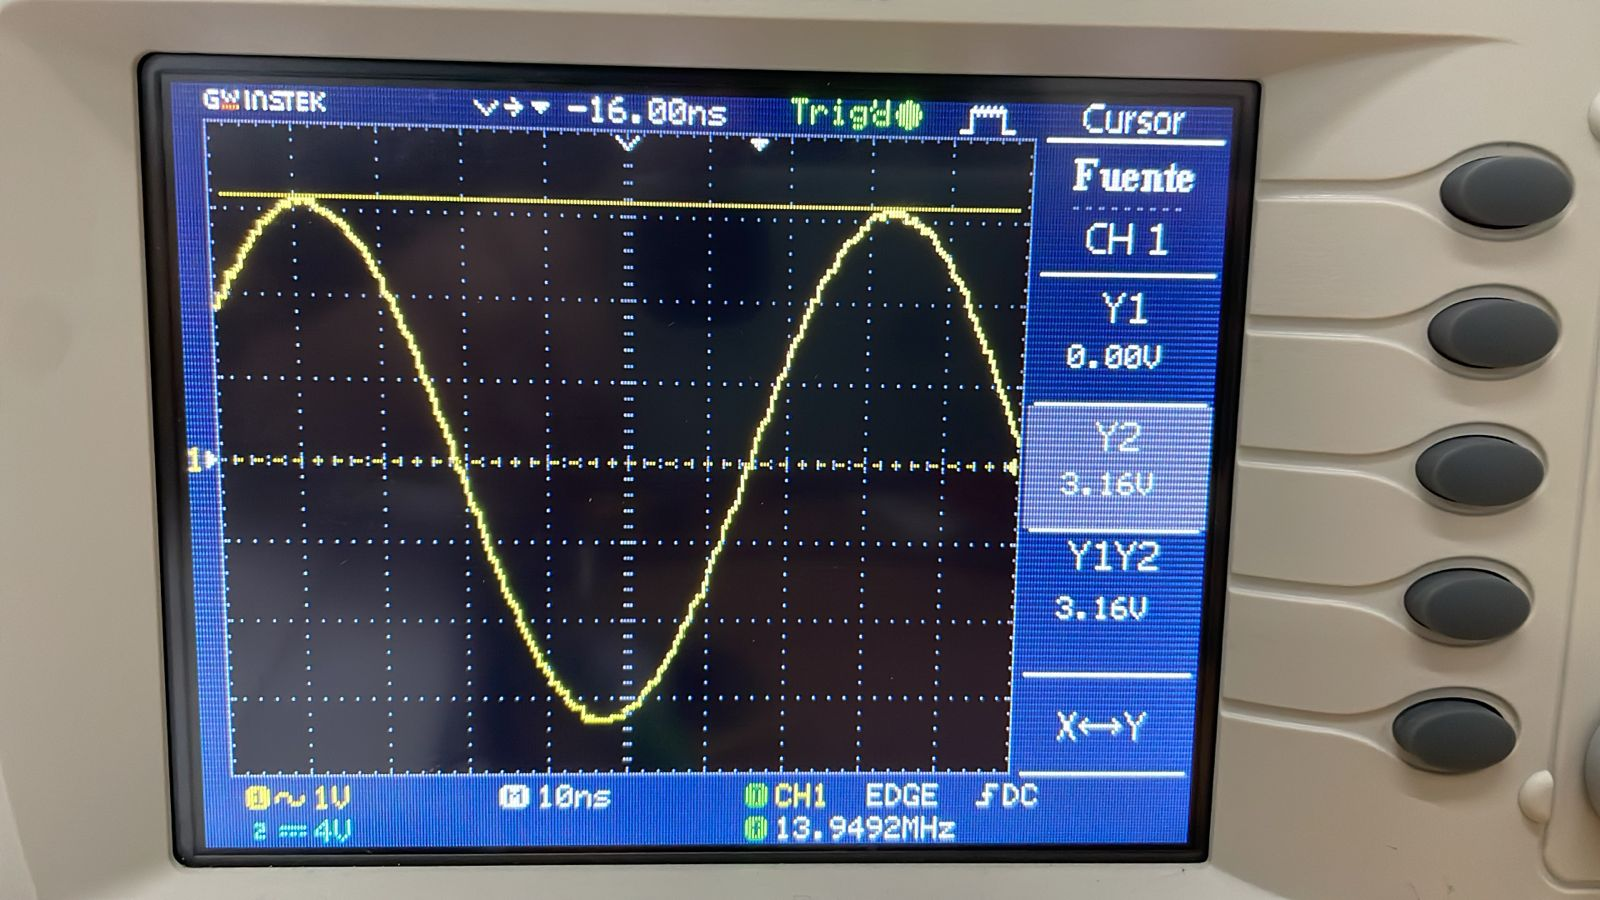
\includegraphics[width=0.8\linewidth]{Figura 20.jpeg}
        \caption{Medición de $Z_{out}$ sin $R_{L}$.}
        \label{fig:fig_20}
    \end{figure}
    
    Mientras que si se observa la Fig. \ref{fig:fig_21} al conectar la carga, la caída de tensión a la salida del circuito es igual a: $V_{x} = 2.24 \ [V]$.

    \begin{figure}[htbp]
        \centering
        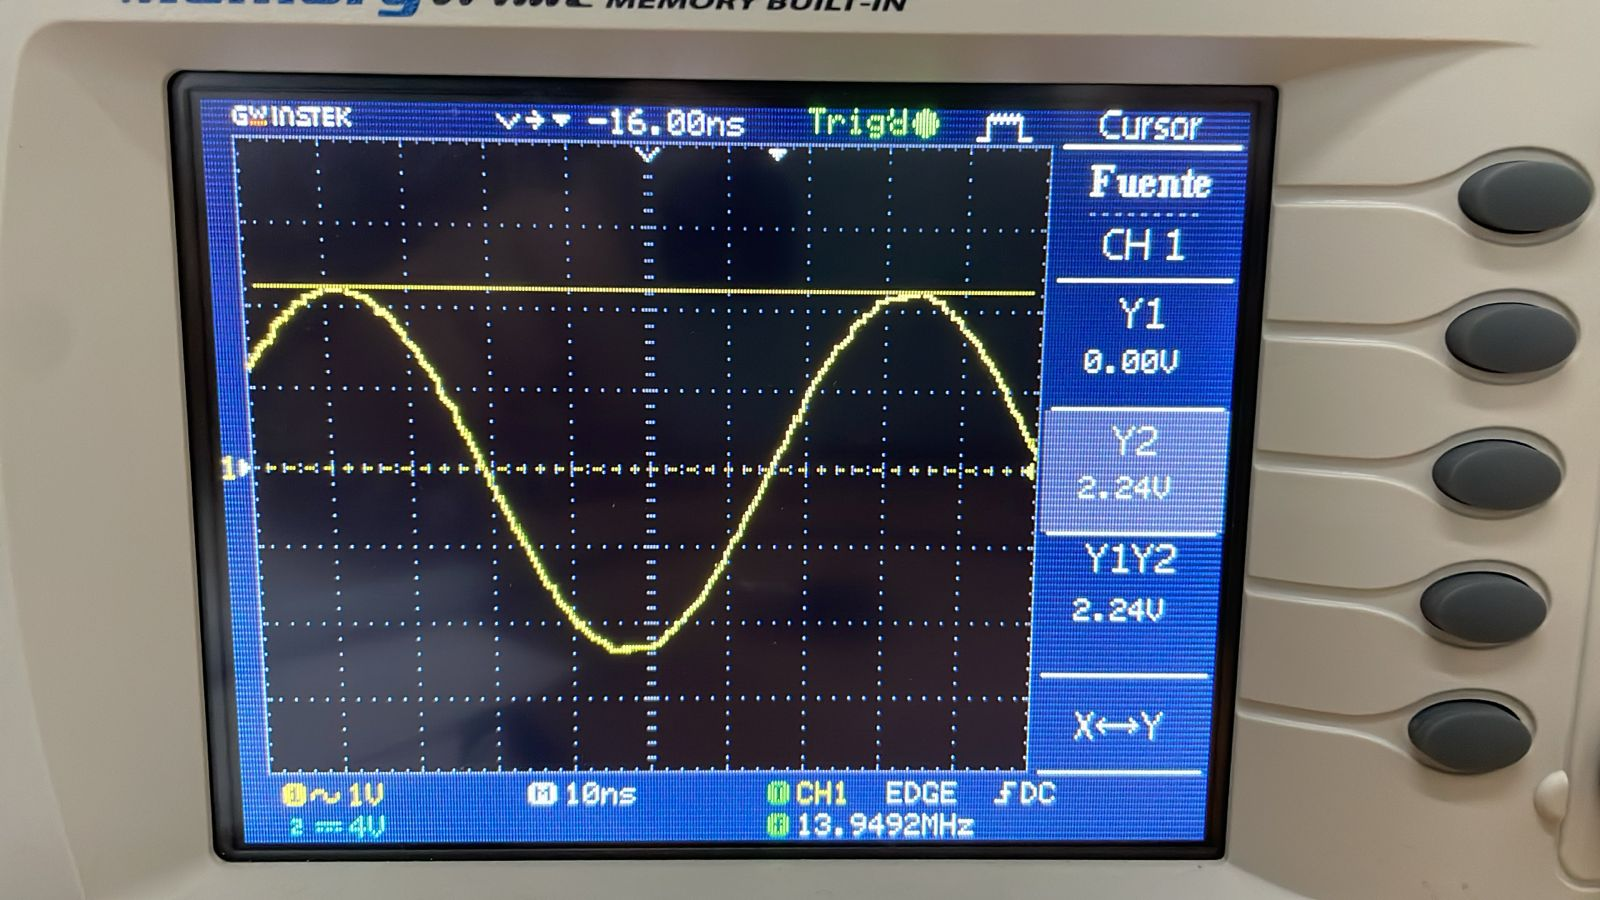
\includegraphics[width=0.8\linewidth]{Figura 21.png}
        \caption{Medición de $Z_{out}$ con $R_{L}$.}
        \label{fig:fig_21}
    \end{figure}

    Aplicando \eqref{eq_38}, se tiene que:
    \begin{equation}
        Z_{out} = \frac{3.16}{2.24}(1000) - 1000 \approx 410.71 \ [\Omega]
        \label{eq_52}
    \end{equation} \\

    \item \underline{Medición de $R_{P}$:} Si bien carece de sentido simular una resistencia de pérdida, resulta totalmente válido realizar la medición física para tener una noción de que tan cercano está el valor real del valor diseñado de esta resistencia. Para ello se debió introducir una resistencia de prueba $R_{test} = 4700 \ [\Omega]$ tal como muestra la Fig. \ref{fig:fig_22}

    \begin{figure}[htbp]
        \centering
        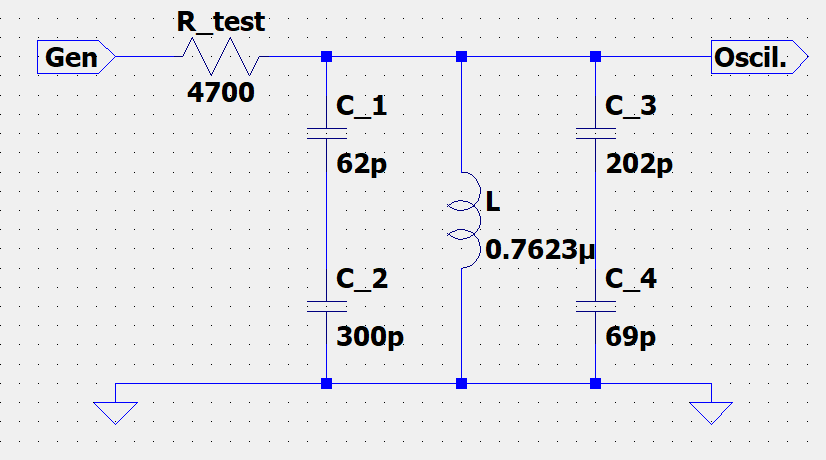
\includegraphics[width=0.8\linewidth]{Figura 22.png}
        \caption{Circuito para la medición de $R_{P}$.}
        \label{fig:fig_22}
    \end{figure}

    Se tiene al no tener carga, en la frecuencia de resonancia las impedancias reactivas se deben anular mutuamente, de modo que la única impedancia en serie con $R_{test}$ será $R_{P}$ y por lo tanto el esquema se simplificó al que muestra la Fig. \ref{fig:fig_23}

    \begin{figure}[htbp]
        \centering
        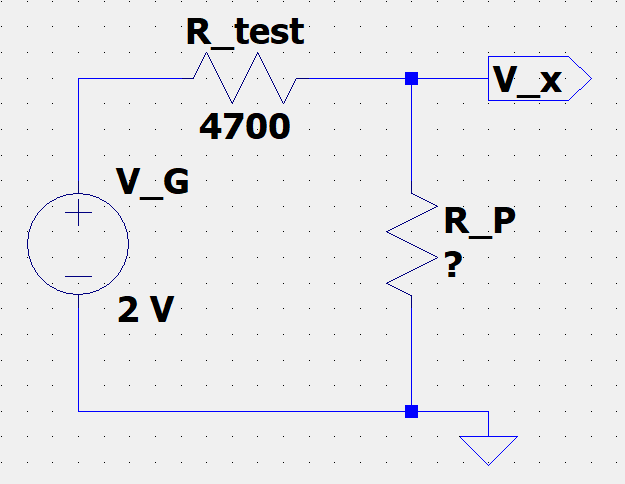
\includegraphics[width=0.5\linewidth]{Figura 23.png}
        \caption{Circuito simplificado para la medición de $R_{P}$.}
        \label{fig:fig_23}
    \end{figure}

    Se tiene que se trata de prácticamente el mismo caso que para medir la impedancia de entrada y por lo tanto, las ecuaciones son las mismas con la salvedad de que se deben cambiar los valores de las variables. 
    En la Fig. \ref{fig:fig_24}, se observa que la tensión $V_{x} = 1.37 \ [V]$ para una alimentación de $V_{G} = 2 \ [V]$.

    \begin{figure}[htbp]
        \centering
        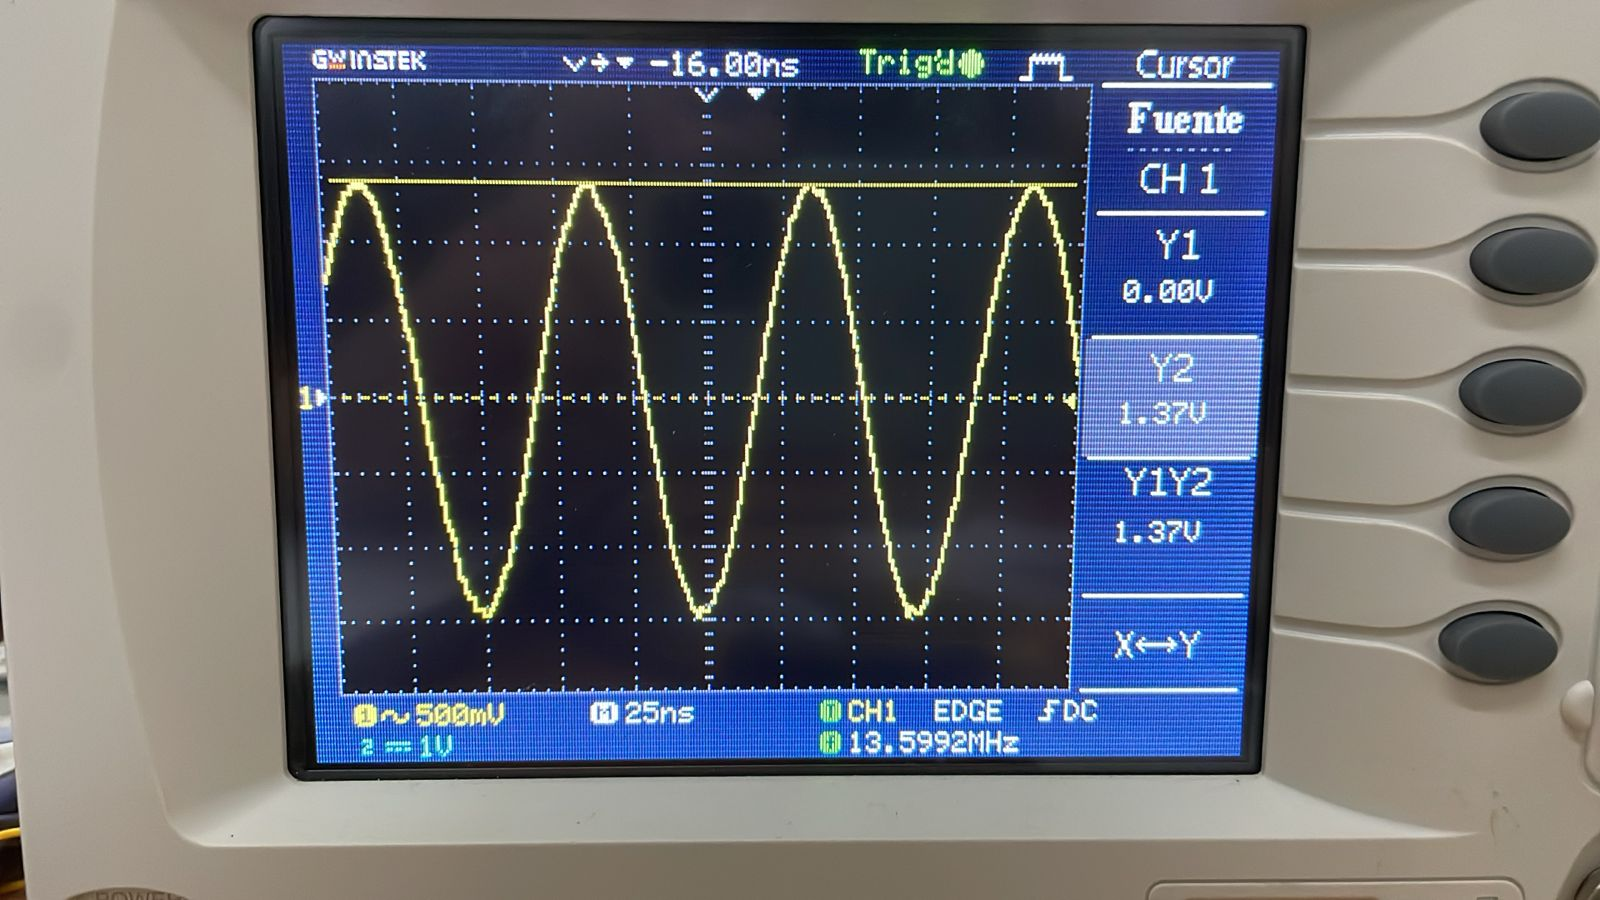
\includegraphics[width=0.8\linewidth]{Figura 24.jpeg}
        \caption{Medición de $R_{P}$.}
        \label{fig:fig_24}
    \end{figure}

    Se deduce según \eqref{eq_34} que:
    \begin{equation}
        R_{P} = \frac{1.37(4700)}{2 - 1.37} \approx 10220.63 \ [\Omega]
        \label{eq_53}
    \end{equation}
\end{itemize}



\section{Conclusión del Acoplador LC paralelo}
Se presenta la Tabla \ref{tab:tab_1}, una comparación los valores obtenidos de diseño, simulación y medición de cada parámetro importante del circuito diseñado, donde ademas se ha realizado una columna extra para representar el error entre lo diseñado y lo simulado.

\begin{table}[htbp]
    \caption{Comparación entre valores calculados, simulados y medidos del acoplador.}
    \centering
    \begin{tabular}{|c|c|c|c|c|} \hline
         \textbf{Variable} & \textbf{Diseño} & \textbf{Simulación} & \textbf{Medición} & \textbf{Error} \\ \hline
         $f_{0} \ [MHz]$      & $18$       & $17.82$  & $17.97$    & $1.00 \ [\%]$     \\ \hline
         $BW \ [MHz]$         & $1.8$      & $1.65$   & $0.8$      & $8.33  \ [\%]$ \\ \hline
         $Z_{in} \ [\Omega]$  & $50$       & $67.64$  & $52.45$    & $35.28 \ [\%]$ \\ \hline
         $Z_{out} \ [\Omega]$ & $1000$     & $670.1$  & $410.71]$  & $32.99\ [\%]$ \\ \hline
         $R_{P}\ [\Omega]$    & $27159.06$ & $-$      & $10220.63$ & $- \ [\%]$ \\ \hline
         $L \ [\mu Hy]$       & $0.7604$   & $0.7604$ & $0.7623]$  & $0.00 \ [\%]$ \\ \hline
    \end{tabular}
    \label{tab:tab_1}
\end{table}

Los valores presentados en la Tabla \ref{tab:tab_1}, son valores que se encuentran dentro de un rango aceptable de diseño. Se tiene que la variación de resultados entre el diseño y la medición se deben principalmente a los aspectos constructivos del inductor, al ajuste de capacitores comerciales realizado, a las capacidades parásitas de los instrumentos de medición, entre otros factores. Por otro lado el error obtenido en las simulaciones con respecto al diseño se debe a la medición realizada con la $R_{P}$ en el circuito de pruebas.



\section{Análisis y Diseño de Acoplamiento $\pi$}
Si bien el análisis y diseño de una red de acoplamiento LC ya se realizó en las secciones precedentes, se incluye aquí una sección extra, en la cual se habla sobre las ecuaciones de diseño de un sistema de acoplamiento con una red $\pi$. Para ello se dividió esta sección en tres partes: las primeras dos tratan sobre el marco teórico empleado y la tercera sobre una aplicación práctica.



\subsection{Nociones Previas al Análisis}
Antes de comenzar el análisis de la red de acoplamiento $\pi$, se deben definir ciertas relaciones útiles que no son propias del acople pero fueron útiles para el desarrollo matemático y diseño propio del acoplador. La primera de ella son las ecuaciones utilizadas para pasar de una red resistiva-reactiva en serie a otra red resistiva-reactiva pero en paralelo tal como muestra la Fig. \ref{fig:fig_25}.

\begin{figure}[htbp]
    \centering
    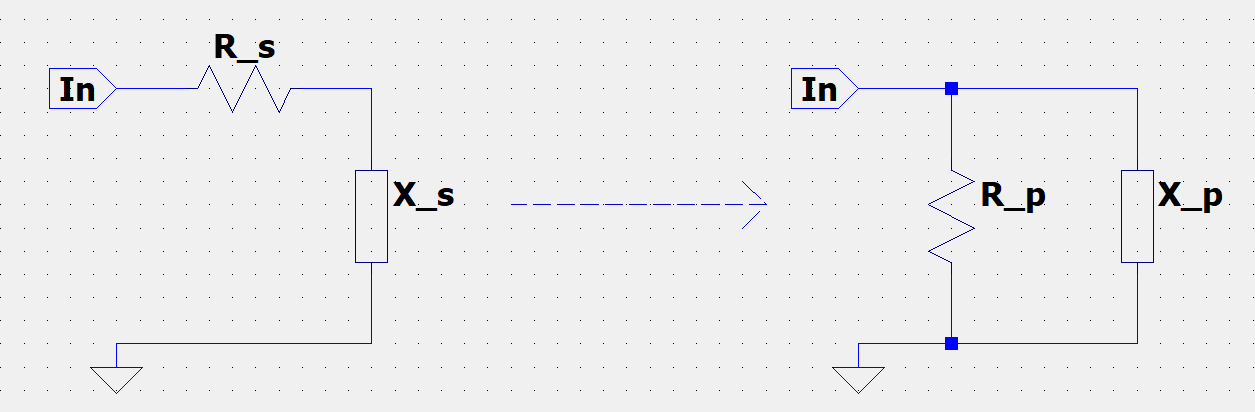
\includegraphics[width=1\linewidth]{Figura 25.png}
    \caption{Pasaje del modelo serie al paralelo de una red resistiva-reactiva genérica.}
    \label{fig:fig_25}
\end{figure}

Realizando un análisis de circuito relativamente simple, se deduce que:
\begin{equation}
    R_{p} = R_{s}\left(1 + \left(\frac{X_{s}}{R_{s}}\right)^2\right) 
    \label{eq_54}
\end{equation}
\begin{equation}
    X_{p} = X_{s}\left(1 + \left(\frac{R_{s}}{X_{s}}\right)^2\right) 
    \label{eq_55}
\end{equation}

Se tiene que una característica fundamental de este pasaje es que el factor de calidad de estos circuitos debe ser exactamente el mismo. Esto se debe a que sólo se ha modificado la forma de representar el circuito, sin embargo los factores de calidad siguen representando el mismo circuito y por lo tanto deben ser iguales. Esto nos lleva a pensar que si los factores de calidad para el modelo serie y paralelo se definen como:
\begin{equation}
    Q_{s} = \frac{X_{s}}{R_{s}}
    \label{eq_56}
\end{equation}
\begin{equation}
    Q_{p} = \frac{R_{p}}{X_{p}}
    \label{eq_57}
\end{equation}

Entonces al tratarse del mismo circuito se tiene que: $Q = Q_{s} = Q_{p}$, tal que operando se dedujo finalmente que:
\begin{equation}
    Q = \sqrt{\frac{R_{p}}{R_{s}}-1}
    \label{eq_58}
\end{equation}

Por otra parte, se tiene que esta red de acoplamiento se conectó entre una etapa amplificadora (compuesta por un transistor BJT de altas frecuencias) y una resistencia de carga $R_{L}$. Dado que ser realizó un análisis en altas frecuencias, el modelo de parámetros híbridos del transistor BJT deja de ser válido por lo que se recurre a un modelo simplificado del transistor que se presenta en la Fig. \ref{fig:fig_26}.

\begin{figure}[htbp]
    \centering
    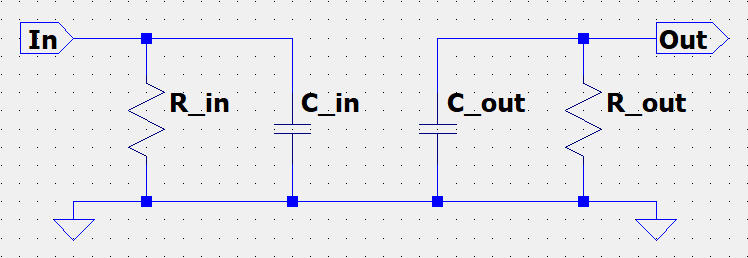
\includegraphics[width=0.9\linewidth]{Figura 26.png}
    \caption{Modelo de impedancias de entrada y salida del transistor BJT.}
    \label{fig:fig_26}
\end{figure}

Este modelo representa al transistor unicamente por sus parámetros de entrada y de salida. Los fabricantes de transistores de altas frecuencias proveen en sus hojas de datos distintas Cartas de Smith mostrando la impedancia compleja de entrada y salida, como líneas de acuerdo a la frecuencia de trabajo del transistor. La Fig. \ref{fig:fig_27} muestra las cartas de Smith mencionadas para un BFP450.

\begin{figure}[htbp]
    \centering
    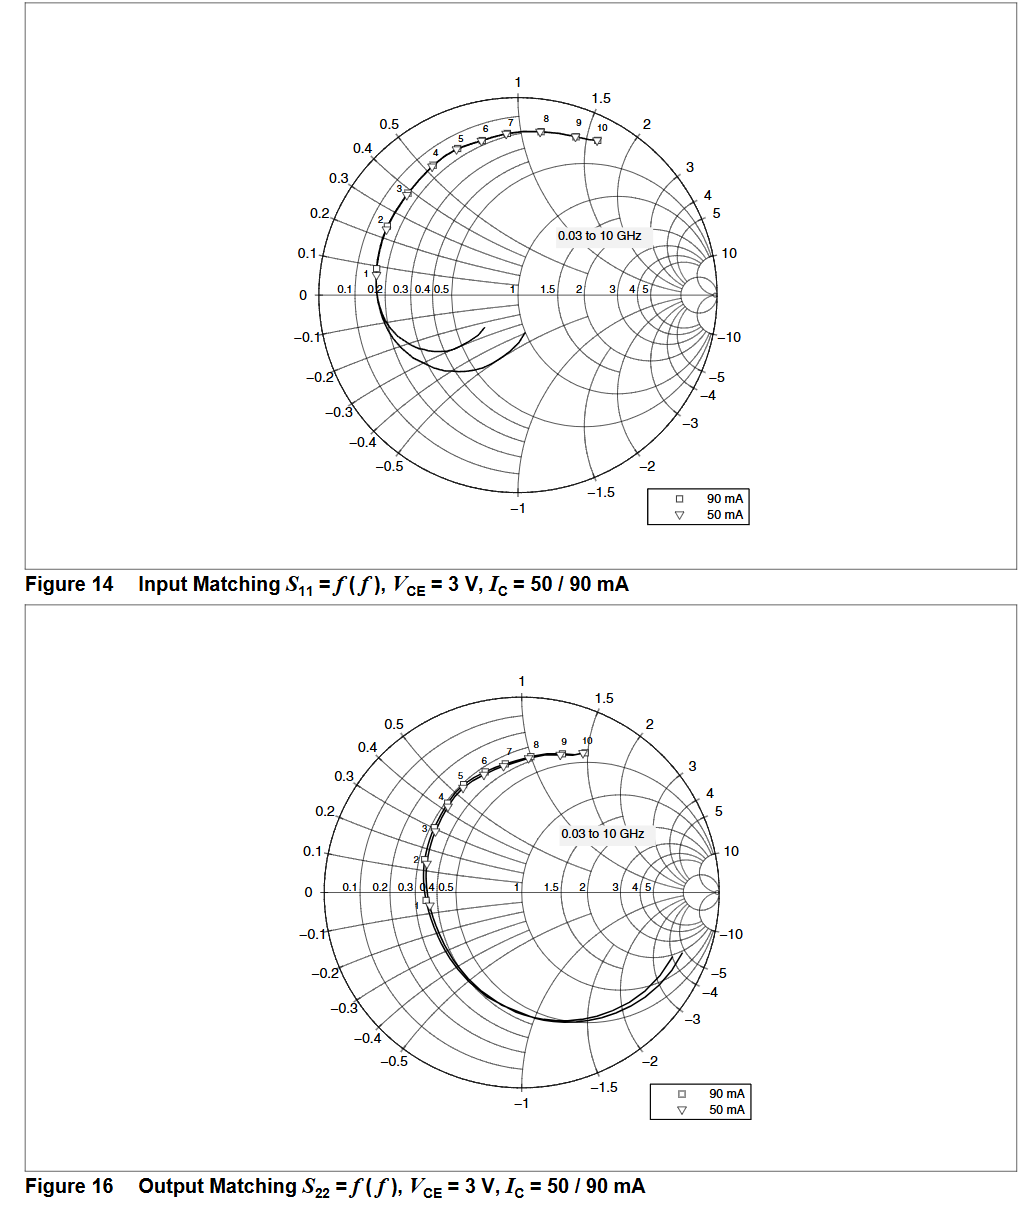
\includegraphics[width=1\linewidth]{Figura 27.png}
    \caption{Impedancias de entrada y salida del \href{https://www.alldatasheet.com/datasheet-pdf/view/415897/INFINEON/BFP450_10.html}{BFP450}. \cite{B6}}
    \label{fig:fig_27}
\end{figure}



\subsection{Análisis del Acoplamiento  $\pi$}
Una red de acoplamiento $\pi$ se caracteriza por tener a sus componentes reactivos dispuestos en un forma de la letra griega en cuestión, tal como se muestra en la Fig. \ref{fig:fig_28} en la cual se ha conectado entre la terminal de salida de un transistor y una resistencia de carga.

\begin{figure}[htbp]
    \centering
    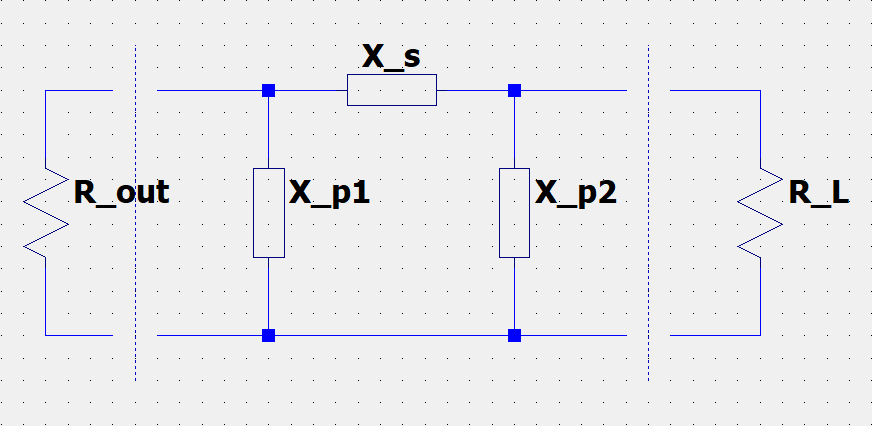
\includegraphics[width=0.9\linewidth]{Figura 28.png}
    \caption{Circuito esquemático del acoplamiento $\pi$.}
    \label{fig:fig_28}
\end{figure}

Se busco en esta sección diseñar un acoplamiento teniendo como datos la frecuencia de resonancia ($f_{0}$), el ancho de banda ($BW$), la resistencia de carga ($R_{L}$) y la resistencia de salida del transistor ($R_{out}$). Nótese aquí que unicamente se trabajo con la resistencia de salida del transistor ya que la reactancia de salida del transistor, se resta o suma a la reactancia paralela del acoplador, dependiendo de su tipo.

Observando la Fig. \ref{fig:fig_28}, se dedujeron los siguientes factores de calidad de los dos circuitos paralelos que forman entre las resistencias y las reactancias paralelas:
\begin{equation}
    Q_{1} = \frac{R_{out}}{X_{p1}}
    \label{eq_59}
\end{equation}
\begin{equation}
    Q_{2} = \frac{R_{L}}{X_{p2}}
    \label{eq_60}
\end{equation}

Luego, se propuso pasar estos pares resistencia-reactancia del modelo paralelo al modelo serie siguiendo \eqref{eq_54} y \eqref{eq_55} tal que el circuito se verá como el siguiente:

\begin{figure}[htbp]
    \centering
    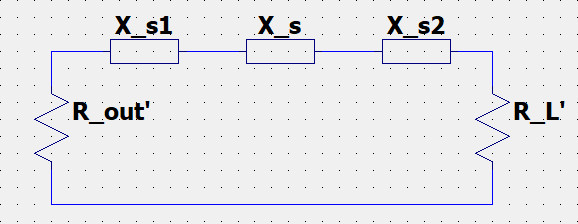
\includegraphics[width=0.9\linewidth]{Figura 29.png}
    \caption{Pasaje del modelo serie al paralelo del acoplamiento $\pi$.}
    \label{fig:fig_29}
\end{figure}

Se definieron entonces los factores de calidad para este circuito serie, los cuales son iguales a los encontrados en \eqref{eq_59} y \eqref{eq_60}.
\begin{equation}
    Q_{1} = \frac{X_{s1}}{R_{out}'}
    \label{eq_61}
\end{equation}
\begin{equation}
    Q_{2} = \frac{X_{s2}}{R_{L}'}
    \label{eq_62}
\end{equation}

Al tratarse de un circuito acoplador, se tiene que este actúa como un filtro pasabanda y por lo tanto debe tener una condición de resonancia. Esto implica que la sumatoria de las reactancias es nula si se usa un generador con frecuencia igual a $f_{0}$, es decir:
\begin{equation}
    X_{s} = (X_{s1} \pm X_{s2})
    \label{eq_63}
\end{equation}

Se utiliza el signo "$\pm$" debido a que se desconoce todavía si estas reactancias serán inductivas o capacitivas. Como se mencionó en el párrafo anterior, al estar en resonancia las impedancias reactivas se anulan entre sí. Luego, dado que buscamos transferir toda la potencia, se tiene que por el teorema de máxima transferencia de energía, las resistencias deben ser iguales, lo que quiere decir que:
\begin{equation}
    R_{tot} = R_{out}' + R_{L}' \implies R_{tot} = 2R_{out}' = 2R_{L}'
    \label{eq_64}
\end{equation}

La idea ahora consistió en poder expresar a las variables $Q_{1}$ y $Q_{2}$ en términos de $Q_{C}$ de modo que de aquí se puedan deducir las reactancias del acoplador. 

Nótese que al estar en resonancia, si se realiza un corte transversal al circuito de la Fig. \ref{fig:fig_29} entre $X_{s}$ y $X_{s2}$, se cumple que las impedancias vistas a cada lado del corte son iguales, de modo que es válido decir que:
\begin{equation}
    Q_{C} = \frac{|X_{s1}| + |X_{s}|}{2R_{tot}'}
    \label{eq_65}
\end{equation}
\begin{equation}
    Q_{C} = \frac{|X_{s2}|}{2R_{L}'}
    \label{eq_66}
\end{equation}

Se observó la similitud entre \eqref{eq_66} y \eqref{eq_62}, de modo que se pudo expresar a $Q_{2}$ en términos de $Q_{C}$ tal que:
\begin{equation}
    Q_{2} = 2Q_{C}
    \label{eq_67}
\end{equation}

Dado que $f_{0}$ y $BW$ son datos de diseño, se puede calcular $Q_{C}$ según \eqref{eq_2}. Consecuentemente, se puede obtener a $X_{p2}$ según \eqref{eq_60} como:
\begin{equation}
    X_{p2} = \frac{R_L}{Q_2}
    \label{eq_68}
\end{equation}

Por otra parte, para obtener el valor de $Q_{1}$ en función de $Q_{C}$, se analizaron los pasajes del modelo paralelo al serie realizados, tal que partiendo de:
\begin{equation}
    R_{L}' = \frac{R_{L}}{1 + \left(\frac{R_{L}}{X_{p2}}\right)^{2}} = \frac{R_{L}}{1 + Q_{2}^{2}}
    \label{eq_69}
\end{equation}
\begin{equation}
    R_{out}' = \frac{R_{out}}{1 + \left(\frac{R_{out}}{X_{p1}}\right)^{2}} = \frac{R_{out}}{1 + Q_{1}^{2}}
    \label{eq_70}
\end{equation}

Se debe cumple que por el teorema máxima transferencia de energía, que estas dos resistencias deben ser iguales y por lo tanto sus expresiones también, de modo que:
\begin{equation}
    \frac{R_{L}}{1 + Q_{2}^{2}} = \frac{R_{out}}{1 + Q_{1}^{2}}
    \label{eq_71}
\end{equation}
\begin{equation}
    1 + Q_{1}^{2} = \frac{R_{out}}{R_{L}}(1 + Q_{2}^{2})
    \label{eq_72}
\end{equation}
\begin{equation}
    Q_{1} = \sqrt{\frac{R_{out}}{R_{L}}(1 + Q_{2}^{2}) - 1}
    \label{eq_73}
\end{equation}

Vemos aquí que todas las variables son datos y por lo tanto, se puede calcular $Q_{1}$. De aquí se pudo calcular a $X_{p1}$ según \eqref{eq_59} tal que:
\begin{equation}
    X_{p1} = \frac{R_{out}}{Q_1}
    \label{eq_74}
\end{equation}

Finalmente, solo restó calcular la reactancia serie $X_{s}$ según \eqref{eq_63} y para ello es necesario obtener los valores serie de las reactancias $X_{s1}$ y $X_{s2}$ para lo cual se usan la relaciones descrita en \eqref{eq_55} tal que:
\begin{equation}
    X_{s1} = \frac{X_{p1}}{1 + \frac{1}{Q_{1}^{2}}}
    \label{eq_75}
\end{equation}
\begin{equation}
    X_{s2} = \frac{X_{p2}}{1 + \frac{1}{Q_{2}^{2}}}
    \label{eq_76}
\end{equation}



\subsection{Ejemplo Práctico} 
Se propone entonces diseñar un acoplador $\pi$ de tipo Colpitts el cual tendrá la topología presentada en la Fig. \ref{fig:fig_30}

\begin{figure}[htbp]
    \centering
    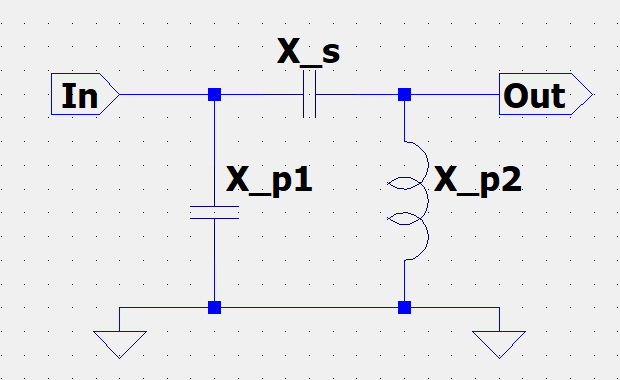
\includegraphics[width=0.6\linewidth]{Figura 30.png}
    \caption{Topología acoplamiento $\pi$ de tipo Colpitts.}
    \label{fig:fig_30}
\end{figure}

Se propone utilizar el transistor BFP450 para la etapa amplificadora, para el cual se consideró que su entrada esta perfectamente adaptada, de modo que los parámetros presentados en la Fig. \ref{fig:fig_27}, sean las impedancias de salida. Se eligió como frecuencia de resonancia una $f_{0} = 1 \ [GHz]$ para la cual se observó que su impedancia normalizada igual a: $\dot{Z_{out}} \approx 0.4 - j0.05$ con $I_{c} = 90 \ [mA]$. Nótese que este valor esta normalizado a $Z_{o} = 50 \ [\Omega]$, tal que des normalizando se deduce que:
\begin{equation}
    Z_{out} = \dot{Z_{out}}(Z_{o}) \approx (0.4 - j0.05)(50) = 20 - j2.5 \ [\Omega]
    \label{eq_77}
\end{equation}
Luego se propuso que: $BW = 30 \ [MHz]$ y que $R_{L} = 50 \ [\Omega]$. Con estos datos en mente, se realizó un cálculo ordenado en forma de pasos simples:
\begin{itemize}
    \item \underline{Paso 1:} Se inició el diseño calculando a $Q_{C}$ según \eqref{eq_2}:
    \begin{equation}
        Q_{C} = \frac{1000 \ [MHz]}{30 \ [MHz]} = 300
        \label{eq_78}
    \end{equation}
    Luego, se tiene que por \eqref{eq_67} que:
    \begin{equation}
        Q_{2} = 2(300) = 600
        \label{eq_79}
    \end{equation}

    \item \underline{Paso 2:} Se calculó a $Q_{1}$ según \eqref{eq_73} tal que:
    \begin{equation}
        Q_{1} = \sqrt{\frac{20}{50}(600^{2}+1)-1} \approx 379.47
        \label{eq_80}
    \end{equation}

    \item \underline{Paso 3:} Se calcularon las reactancias paralelo siguiendo \eqref{eq_74} y \eqref{eq_68} tal que:
    \begin{equation}
        X_{p1} = \frac{20}{379.47} \approx 0.0527 \ [\Omega]
        \label{eq_81}
    \end{equation}
    \begin{equation}
        X_{p2} = \frac{50}{600} \approx 0.0833 \ [\Omega]
        \label{eq_82}
    \end{equation}
    De aquí se pudieron deducir los valores de capacitancia e inductancia de las ramas paralelo del circuito. Se comenzó calculando la capacitancia en $X_{p1}$ a la cual se le consideró el efecto que tiene el capacitor a la salida del transistor, es decir:
    \begin{equation}
        C_{p1} =  \frac{1}{2\pi f_{0}(X_{p1})} - \frac{1}{2\pi f_{0}(X_{out})}
        \label{eq_83}
    \end{equation}
    \begin{equation}
        C_{p1} = \frac{1}{2\pi(1x10^{9})(0.0527)} - \frac{1}{2\pi(1x10^{9})(2.5)}
        \label{eq_84}
    \end{equation}
    \begin{equation}
        C_{p1} \approx  2.95 \ [nF]
        \label{eq_85}
    \end{equation}
    Luego para el inductor en $X_{p2}$, se tiene que:
    \begin{equation}
        L_{p2} = \frac{X_{p2}}{2\pi f_{0}} = \frac{0.0833}{2\pi(1x10^{9})}
        \label{eq_86}
    \end{equation}
    \begin{equation}
        L_{p2} \approx  13.25 \ [pHy]
        \label{eq_87}
    \end{equation}

    \item \underline{Paso 4:} Para calcular la reactancia serie, se necesitó utilizar la condición de resonancia de \eqref{eq_63} y para ello se necesitaron calcular las reactancias serie $X_{s1}$ y $X_{s2}$ según \eqref{eq_75} y \eqref{eq_76}. Tal que:
    \begin{equation}
        X_{s1} = \frac{0.0527}{1 + \frac{1}{(379.47)^{2}}} \approx 0.0526 \ [\Omega]
        \label{eq_88}
    \end{equation}
    \begin{equation}
        X_{s2} = \frac{0.0833}{1 + \frac{1}{(600)^{2}}} \approx 0.0832 \ [\Omega]
        \label{eq_89}
    \end{equation}

    \item \underline{Paso 5:} Reemplazando lo obtenido en el paso anterior en \eqref{eq_63} se tiene que:
    \begin{equation}
        X_{s} = 0.0832 - 0.0526 \approx 0.0306 \ [\Omega]
        \label{eq_90}
    \end{equation}
    Se dedujo finalmente que el valor de la capacitancia $C_s$ es igual a:
    \begin{equation}
        C_{s} = \frac{1}{2\pi(1x10^{9})(0.0306)}
        \label{eq_91}
    \end{equation}
    \begin{equation}
        C_{s} \approx 5.20 \ [nF]
        \label{eq_92}
    \end{equation}
\end{itemize}

Para concluir con este apartado, se propuso simular el circuito en LTSpice con los valores obtenidos para el acoplador $\pi$. En la Fig. \ref{fig:fig_31} se presenta el circuito a simular.

\begin{figure}[htbp]
    \centering
    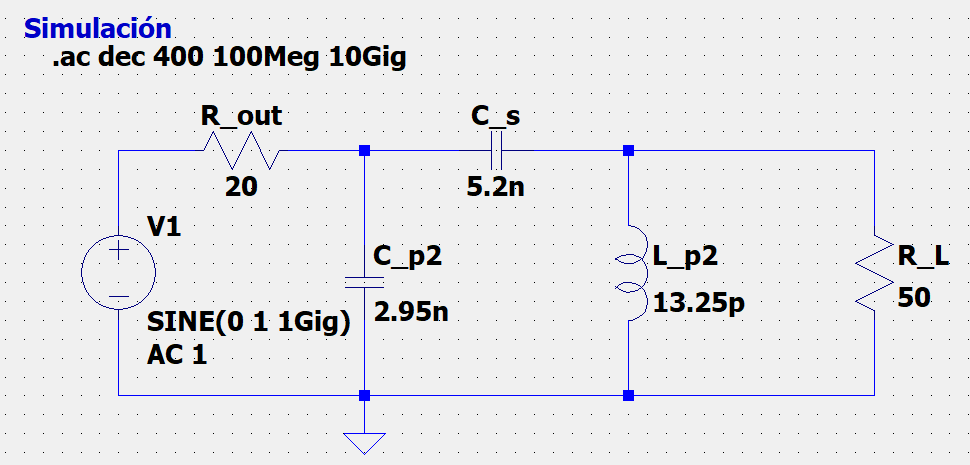
\includegraphics[width=0.8\linewidth]{Figura 31.png}
    \caption{Simulación en LTSpice del acoplamiento $\pi$.}
    \label{fig:fig_31}
\end{figure}

Si realizamos un análisis en AC, se pudo medir la frecuencia de resonancia $f_{0}$ la cual se observa en la Fig. \ref{fig:fig_32}.

\begin{figure}[htbp]
    \centering
    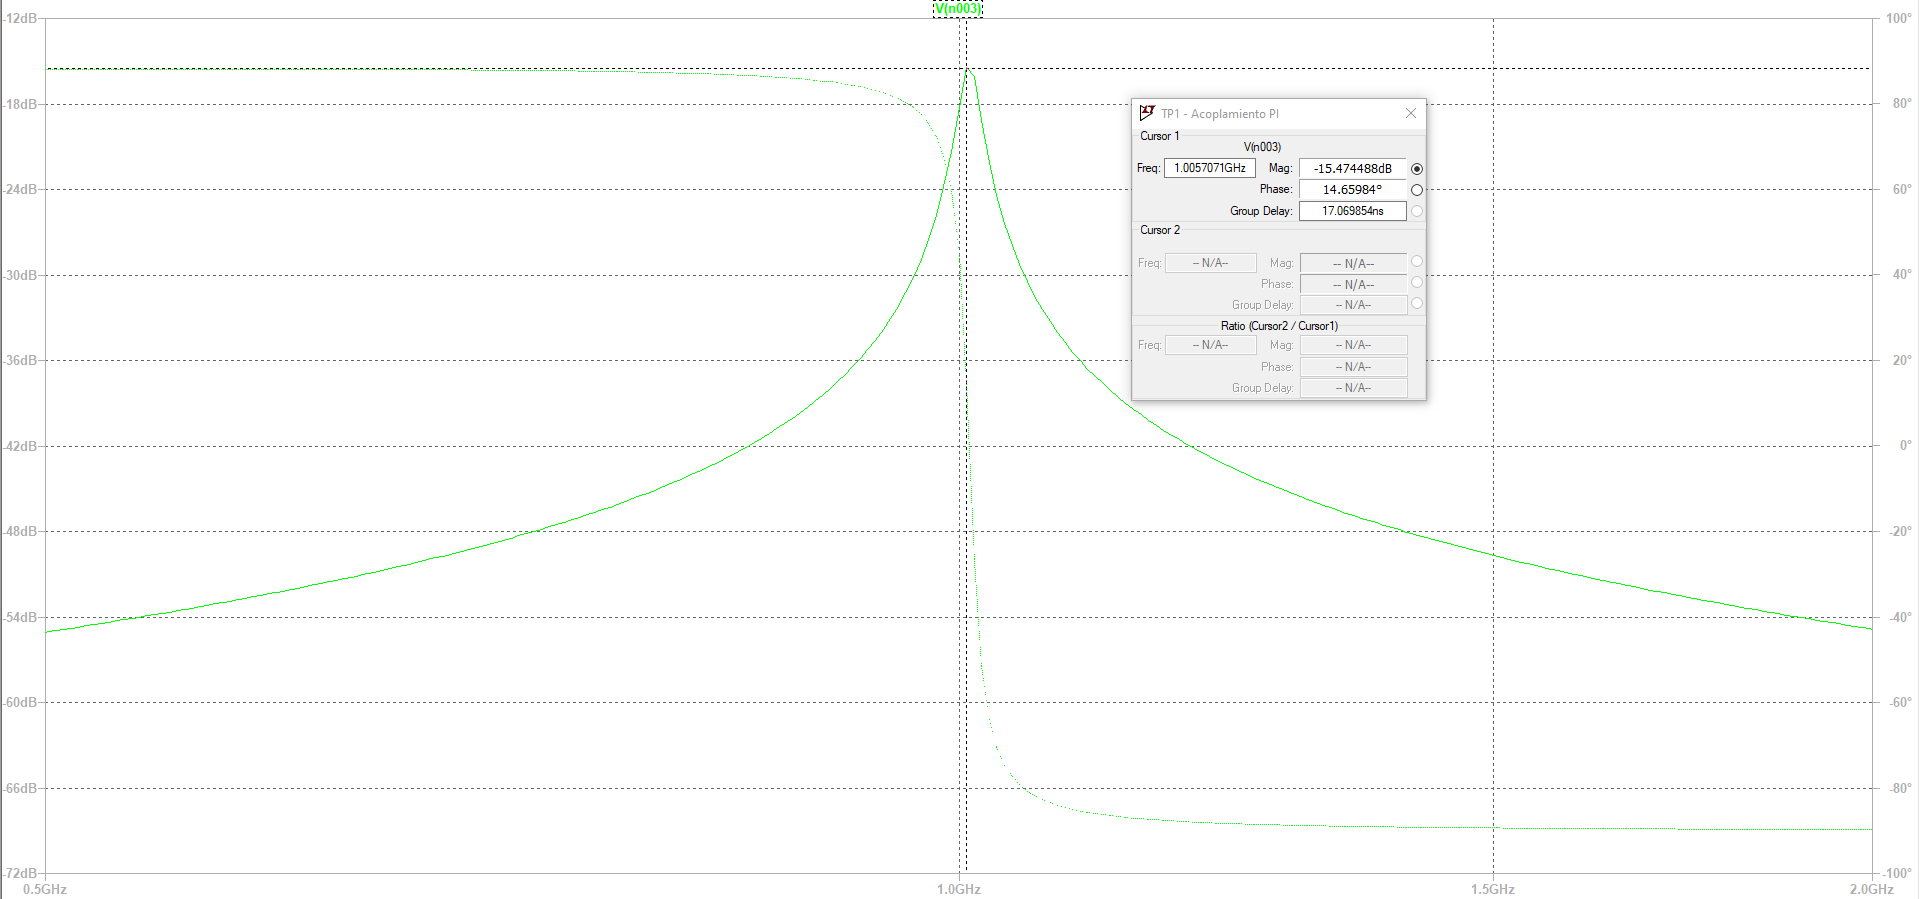
\includegraphics[width=0.8\linewidth]{Figura 32.png}
    \caption{Medición de $f_{0}$ del acoplamiento $\pi$.}
    \label{fig:fig_32}
\end{figure}

Se observa que $f_{0} = 1.0057 \ [GHz]$ lo que muestra un correcto calculo y diseño de este tipo de acoplamiento.



\section{Conclusiones Finales}
A modo de conclusión, se ha demostrado a lo largo de este informe un procedimiento claro y detallado sobre como diseñar una red de acoplamiento LC paralela: Para ello se planteó un marco teórico, seguido de un diseño por software utilizando Python para diseñar el inductor y los capacitores; Luego se simuló el circuito en LTSpice previo al armado para verificar que los valores obtenidos eran próximos a los del diseño. Finalmente se procedió con el armado y medición física del circuito en donde se obtuvieron mediciones bastante cercanas a las esperadas, concluyendo así con el análisis y diseño de esta red LC paralela para un acople inter-etapa de radiofrecuencias.

Además, se realizó un apartado extra donde se analizo las ecuaciones de diseño de un acoplamiento $\pi$ siguiendo el mismo marco teórico, donde además se realizó tanto el cálculo como la verificación por simulación en LTSpice, del circuito diseñado con valores reales de componentes, tales como el transistor BFP450.



\section{Bibliografía}
Si desea consultar más información al respecto, se recomienda revisar el repositorio de \href{https://github.com/ErnestMonja/Electronica_Analogica_III/tree/main/Trabajo%20Pr%C3%A1ctico%20N%C2%B01%20-%20Circuitos%20Sintonizados}{GitHub} donde se incluye el Script de Python para el diseño de los inductores y capacitores, los archivos de simulación en LTSpice y los archivos en \LaTeX $\ $ de este informe.

A continuación, se presenta la lista de referencias de acuerdo a las citaciones mencionadas a lo largo de este trabajo practico con hipervínculos incluidos:

\begin{thebibliography}{00}
    \bibitem{B1} Chapman, S. J. (2012). \textit{Máquinas Eléctricas} (5ta ed., pp. 47-117). McGraw-Hill Education. \href{https://frrq.cvg.utn.edu.ar/pluginfile.php/20762/mod_resource/content/1/Maquinas-electricas-Chapman-5ta-edicion-pdf.pdf}{https://frrq.cvg.utn.edu.ar/Maquinas-electricas-Chapman}
    \bibitem{B2} Monja, E. J. (2026). \textit{Script de Inductor-Capacitores (Final)} [Software]. GitHub. \href{https://github.com/ErnestMonja/Electronica_Analogica_III/blob/main/Trabajo%20Pr%C3%A1ctico%20N%C2%B01%20-%20Circuitos%20Sintonizados/TP1%20-%20Script%20de%20Inductor-Capacitores%20(Final).ipynb}{https://github.com/ErnestMonja/Electronica\_Analogica\_III}
    \bibitem{B3} Wikipedia. (s.f.). \textit{Slide (guitarra)}. Recuperado el 9 de abril de 2026, de \href{https://es.wikipedia.org/wiki/Slide_(guitarra)}{https://es.wikipedia.org/wiki/Slide\_(guitarra)}
    \bibitem{B4} Cátedra de Tecnología Electrónica. (s.f.). \textit{Apuntes sobre la Constante de Nagaoka}. [Material de clase]. Universidad Nacional de Córdoba.
    \bibitem{B5} Ingenio Triana. (2, de noviembre de 2016). \textit{Diseño de inductores: cálculo de bobinas y fórmula de Wheeler}. \href{https://ingenio-triana.blogspot.com/2016/11/diseno-de-inductores-calculo-de-bobinas_2.html}{https://ingenio-triana.blogspot.com}
    \bibitem{B6} Infineon Technologies. (s.f.). \textit{BFP450: Surface Mount Silicon Germanium Carbon NPN RF Transistor} [Hoja de datos]. \href{https://www.alldatasheet.com/datasheet-pdf/view/415897/INFINEON/BFP450_10.html}{https://www.alldatasheet.com}
\end{thebibliography}



\end{document}
